\documentclass[fontsize=11pt,paper=a4,lualatex]{jlreq}

%% パッケージ
\usepackage{amsmath,amssymb,amsthm}
\usepackage{booktabs,array,longtable}
\usepackage{graphicx}
\graphicspath{{supplementary/}}
\usepackage{hyperref}
\usepackage{needspace}
\usepackage{luatexja}
\usepackage[match]{luatexja-fontspec}

%% フォント設定
\setmainfont{Latin Modern Roman}
\setmainjfont[
  BoldFont = Noto Sans CJK JP Bold
]{Noto Serif CJK JP}
\setsansjfont{Noto Sans CJK JP}

%% Paper II マーク（該当主張の厳密化は Paper II が与える；§1で一度だけ宣言）
\newcommand{\PII}{\textsuperscript{\textup{II}}}

%% Unicode数学記号（本文中で使用）
\usepackage{newunicodechar}
\newunicodechar{α}{\ensuremath{\alpha}}
\newunicodechar{β}{\ensuremath{\beta}}
\newunicodechar{δ}{\ensuremath{\delta}}
\newunicodechar{ε}{\ensuremath{\varepsilon}}
\newunicodechar{θ}{\ensuremath{\theta}}
\newunicodechar{κ}{\ensuremath{\kappa}}
\newunicodechar{λ}{\ensuremath{\lambda}}
\newunicodechar{μ}{\ensuremath{\mu}}
\newunicodechar{ν}{\ensuremath{\nu}}
\newunicodechar{π}{\ensuremath{\pi}}
\newunicodechar{ρ}{\ensuremath{\rho}}
\newunicodechar{σ}{\ensuremath{\sigma}}
\newunicodechar{τ}{\ensuremath{\tau}}
\newunicodechar{φ}{\ensuremath{\phi}}
\newunicodechar{ψ}{\ensuremath{\psi}}
\newunicodechar{χ}{\ensuremath{\chi}}
\newunicodechar{Σ}{\ensuremath{\Sigma}}
\newunicodechar{Ω}{\ensuremath{\Omega}}
\newunicodechar{Λ}{\ensuremath{\Lambda}}
\newunicodechar{Δ}{\ensuremath{\Delta}}
\newunicodechar{∈}{\ensuremath{\in}}
\newunicodechar{≠}{\ensuremath{\neq}}
\newunicodechar{≡}{\ensuremath{\equiv}}
\newunicodechar{≥}{\ensuremath{\geq}}
\newunicodechar{≤}{\ensuremath{\leq}}
\newunicodechar{→}{\ensuremath{\to}}
\newunicodechar{×}{\ensuremath{\times}}
\newunicodechar{≈}{\ensuremath{\approx}}
\newunicodechar{∝}{\ensuremath{\propto}}
\newunicodechar{±}{\ensuremath{\pm}}
\newunicodechar{∞}{\ensuremath{\infty}}
\newunicodechar{⊗}{\ensuremath{\otimes}}
\newunicodechar{∂}{\ensuremath{\partial}}
\newunicodechar{∼}{\ensuremath{\sim}}
\newunicodechar{≅}{\ensuremath{\cong}}
\newunicodechar{≪}{\ensuremath{\ll}}
\newunicodechar{□}{\ensuremath{\square}}
\newunicodechar{ℂ}{\ensuremath{\mathbb{C}}}
\newunicodechar{ℝ}{\ensuremath{\mathbb{R}}}
\newunicodechar{ℤ}{\ensuremath{\mathbb{Z}}}
\newunicodechar{₀}{\ensuremath{_0}}
\newunicodechar{₁}{\ensuremath{_1}}
\newunicodechar{₂}{\ensuremath{_2}}
\newunicodechar{₃}{\ensuremath{_3}}
\newunicodechar{₉}{\ensuremath{_9}}
\newunicodechar{²}{\ensuremath{^2}}
\newunicodechar{³}{\ensuremath{^3}}
\newunicodechar{⁴}{\ensuremath{^4}}
\newunicodechar{⁵}{\ensuremath{^5}}
\newunicodechar{⁶}{\ensuremath{^6}}
\newunicodechar{⁻}{\ensuremath{^{-}}}
\newunicodechar{¹}{\ensuremath{^1}}
\newunicodechar{⁰}{\ensuremath{^0}}
\newunicodechar{−}{\ensuremath{-}}
\newunicodechar{✓}{\checkmark}
\newunicodechar{∩}{\ensuremath{\cap}}
\newunicodechar{∫}{\ensuremath{\int}}
\newunicodechar{⟨}{\ensuremath{\langle}}
\newunicodechar{⟩}{\ensuremath{\rangle}}

%% hyperref設定
\hypersetup{
  colorlinks=true,
  linkcolor=blue,
  citecolor=blue,
  urlcolor=blue,
  pdftitle={存在からの物理学 I: The Equation},
  pdfauthor={近藤秀和},
  pdfsubject={存在からの物理学},
  pdfkeywords={物理学, 標準模型, 情報幾何, エントロピー, 存在}
}

%% 定理環境
\newtheorem{theorem}{定理}

%% jlreq見出し設定（プロフェッショナルなスタイル）
\jlreqsetup{
  caption_label_format={#1.},
  caption_font={\normalfont\small},
  caption_label_font={\normalfont\small\bfseries},
}

%% タイトル
\title{\textbf{存在からの物理学 I: The Equation}\\[0.45em]{\large 二値エントロピー方程式 $V = -H$ と標準模型パラメータの構造}}
\author{近藤秀和\\[0.5em]\small\textit{東京}}
\date{2026年4月}

\begin{document}
\maketitle
\begin{abstract}\sloppy\noindent\label{ux6982ux8981}

標準模型の26個の自由パラメータを同時に導出した理論は存在しない。本論文では、存在に関する3つの公理---存在は二値的である（$n \in \{0,1\}$、すなわち $n^2{=}n$）、存在は不確実である（$\sigma \neq 1$）、非存在は禁止される（$\sigma \neq 0$）---から単一の方程式 V = −H が代数的恒等式として定まることを示す。この方程式が生み出す数学的構造は標準模型の構造と対応し、20以上の物理量が調整可能なパラメータなしに再現され、全て 0.0006\%--2.6\% の精度で実験と一致する。

V = −H は二値自由度 n ∈ \{0,1\}
の正準自由エネルギーであり、フェルミ・ディラック分布の Legendre
変換により定まる。このポテンシャルと正準規格化（$g = 1$、\S2.4）の運動項により、シュレーディンガー方程式が転送行列として導出される。この方程式はちょうど3つの束縛状態（離散解）を持ち、それがフェルミオンの3世代に対応する。空間次元
d = 3
は井戸の保存・スピン統計・重力伝播の3条件から導かれる。この一致から展開される数学的構造がゲージ群
SU(3)×SU(2)×U(1) を再現する。

この構造から、1/α = 137.0368（0.0006\%）、$\alpha_s$ = 0.1179（0.01\%）、$\sin^2\!\theta_W$ = 3/13（0.2\%）、荷電レプトン質量比 R =
1.5293（0.006\%）、$\sin\theta_C$ = 0.2245（0.10\%）を含む20以上の物理定数が導かれる。さらにニュートリノの絶対質量（$\Sigma m_\nu$ = 59.2 meV）、ニュートリノなし二重ベータ崩壊の厳密なゼロを含む7つの検証可能な予測を与える。これらの量は独立な入力パラメータではなく、すべて V = −H により定まる同一の数学的構造から計算される。

\end{abstract}

\section{導入}\label{ux5c0eux5165}

標準模型は素粒子物理学の最も成功した理論である。既知の全ての素粒子相互作用を記述し、ヒッグス粒子の発見
\cite{atlas,cms}（2012）を含む膨大な実験的検証に耐えてきた。しかしこの理論は
26 個の自由パラメータを含む\footnote{質量ゼロのニュートリノを仮定する最小標準模型では19個；ニュートリノ質量3個とPMNSパラメータ4個を加えて26個。$v_\mathrm{EW}$ をエネルギースケールに吸収して25と数える文献もある。}---フェルミオン質量（Yukawa
結合定数）、混合角、ゲージ結合定数、ヒッグスの自己結合、そして CP
位相。これらの値は実験から測定して入力するしかなく、なぜそれらの値を取るのかは標準模型の中では説明されない。世代数
N = 3
もまた説明のない入力である。大統一理論（GUT）、超対称性（SUSY）、弦理論などの多くの試みにもかかわらず、26
個全てのパラメータを同時にゼロ自由パラメータで決定した理論は存在しない
\cite{xing}。微細構造定数 $\alpha$ という1個の定数ですら、第一原理からの導出の試み~\cite{eddington, wyler, jentschura} には長い歴史があるが、統一的な方程式や機構を欠いた孤立した数値的一致にとどまってきた。

情報理論から物理を導くという別のアプローチも試みられてきた。Wheeler の「it from bit」\cite{wheeler} は物理的実在が情報から生まれるという構想を提唱したが、数学的枠組みを持たなかった。Jaynes \cite{jaynes} はエントロピー最大化から統計力学を導出したものの、場の量子論には至らなかった。Verlinde \cite{verlinde} はエントロピー的推論から重力を導出したが、対象は重力のみにとどまった。このほか Frieden \cite{frieden} の Fisher 情報アプローチ、Caticha \cite{caticha} の情報幾何、Hardy \cite{hardy} と Chiribella ら \cite{chiribella} の情報論的公理化がある。これら全てのアプローチは共通の限界を持つ：物理方程式の\emph{形式}は導出できても、そこに現れる定数の\emph{値}は導出できないことである。精神において最も近い先行研究は Connes--Chamseddine のスペクトル標準模型~\cite{connes96,chamconnes96,ccm07} であり、非可換幾何の代数構造から標準模型のゲージ群・Higgs セクター・パラメータ関係を導く。同模型がパラメータなしで予言した $m_H \approx 170$ GeV は実験で反証され、後に singlet 場の追加で修復された---パラメータフリーな質量予言に対する直接の教訓であり、本論文の予言にも同じ基準が適用される。関連する代数的再構成として Furey の分割代数アプローチ~\cite{furey} がある。

本論文は3つの公理を出発点とする：存在（$n \in \{0,1\}$）、不確実性（$\sigma \neq 1$）、非存在の禁止（$\sigma \neq 0$）。A2 と A3 を合わせて $\sigma \in (0,1)$、分配関数 $Z = 1 + e^{\phi}$、そして Fermi--Dirac 分布の Legendre 変換により正準自由エネルギー $V = -H(\sigma(\phi))$ が代数的恒等式として定まる。ここで $H$ は2値 Shannon エントロピー、$\sigma(\phi)$ は Fermi--Dirac 分布（シグモイド関数）、$\phi = \mathrm{logit}(\sigma)$ は自然パラメータ~\cite{amari,ay} である。このポテンシャルと、正準規格化（$g = 1$、\S2.4）の運動項により、シュレーディンガー方程式が転送行列として導出される。

このシュレーディンガー方程式はちょうど3つの束縛状態を持ち（N =
3）、フェルミオンの3世代に対応する。空間次元 d = 3 が井戸の保存・スピン統計・重力伝播の3条件から、時空次元 D = 4 が重力自由度マッチングと ℂP² から、シグネチャ (3,1) が $M_2(\mathbb C)_{\mathrm{sa}}$ の構造への接続として従う（§4、§9）。ゲージ構造 PG(2, F₃) は N = d = 3 の一致から展開される数学的構造であり、ゲージ群 SU(3)×SU(2)×U(1) と一意に構造が対応する。ゲージ群の表現から 48 フェルミオン・12 ゲージボソン・1 ヒッグスの全粒子を導く構造が導出される（§5）。この構造から20以上のパラメータが導かれる---$1/\alpha_{\mathrm{em}}$ = 137.0368（0.0006\%）、$\sin^2\!\theta_W$ = 3/13（0.2\%）、荷電レプトン質量比 R = 1.5293（0.006\%）、Koide の Q ≈ 3/2（δ = −1.5 × 10⁻⁵）、CKM/PMNS 混合角---全て自由パラメータなしに 0.0006\%--2.6\% の精度で実験と一致する（§10）。関連する Paper~II の再構成はさらに matching 点の条件 $\bar\theta(\mu_0)=0$\PII{} を与えるが、これは V-パリティ単独の帰結ではない。

数値的な一致に加え、$V = -H$ から導かれる数学的構造は、標準模型の構造的問題に対応する。標準模型で $\mu^2 > 0$ が果たす役割---真空を対称点から有限の場の値へ移すこと---を $V$ の井戸の形状が担い（§7）、内部ポテンシャルが有界（$V \in [-\ln 2, 0]$）であることは不安定性チャンネルを与えず、準安定性問題も階層性問題もこの構成内では生じない（4D の真空安定性・階層性問題との対応は再構成マッチングを要する）。$V = -H$ は $n \in \{0,1\}$ の正準自由エネルギーとして一意であるため、ヒッグスは1つに定まる。

なお、本論文が示すのは、$V = -H$ から生じる数学的構造を標準模型の構造に対応させたとき、導出される数値が実験値と一致することであり、標準模型そのものを第一原理から厳密に導出するものではない。また、方程式の展開だけでは決まらない選択---各観測量を構造のどの分率・どの演算子・どの係数で読み取るか---が随所に現れる。本論文はその選択（読み出しの指定）を明示した上で数値を計算する。各選択が自由なパラメータではないこと、すなわちその一意性と剛性の証明、および本論文の各構成の演算子レベルの導出は Paper~II~\cite{paper2} が与える。本文では個別に再掲しない。

本論文の構成は以下の通りである。§2 で3つの公理から $V = -H$
を導出し、シュレーディンガー方程式を確立する。§3 で束縛状態数 $N = 3$
を数学的定理として証明する。§4 で空間次元 $d = 3$
を三つの独立な実現整合条件の共通解として導く。§5 で PG(2,3)
のゲージ構造を構成する。§6 でゲージ結合定数を導出する。§7 でヒッグス質量を導き、真空の内部点固定と内部ポテンシャルの有界性（不安定性チャンネルなし）を示す。§8 で束縛状態を荷電レプトンの3世代に対応させ、フェルミオンの質量と混合を導く。§9 で時空次元 $D = 4$ とシグネチャ $(3,1)$ を前提を置いた整合性検査により確認し、構成の独立性からテンソル積構造 $\mathcal{H}_\mathrm{int}(\phi) \otimes \mathcal{H}_\mathrm{space}(x)$ を確立する。§10
で全結果をまとめ、反証可能な予測を提示する。§11 で結論を述べる。



\section{存在から方程式へ}\label{ux5b58ux5728ux304bux3089ux65b9ux7a0bux5f0fux3078}

本章では、存在についての3つの公理を数学的に定式化し、代数的変換により基本方程式 V = −H を導出する。この方程式から標準模型と整合する構造が現れる。

\subsection{公理}\label{ux516cux7406}

本論文の全構造の基礎となる3つの公理を定義する。

\textbf{A1（存在）：} 何かが存在する。「存在する」は命題であり、真か偽のいずれかである---排中律により第三の値はない。存在の状態を $n$ と書けば、状態空間は $n \in \{0,1\}$ である。A1 は状態空間を定めるが $n$ の\textbf{値}は定めない。

\textbf{A2（不確実性）：} 存在は不確実である。存在するものは何であれ、確実には存在しない。占有確率を $\sigma = \langle n \rangle$ と書けば、$\sigma \neq 1$。A2 は上端（確実な存在）を除外するが、下端については何も言わない。

\textbf{A3（非存在の禁止）：} 非存在は状態ではない（$\sigma \neq 0$）。在ることの欠如である在り方は矛盾である。

これら3つの公理から、標準模型の構造と定数が従う。以下でこれを形式化する。

\subsection{二値性と分配関数}\label{ux4e8cux5024ux6027}

A1 が定めた状態空間 $n \in \{0,1\}$ から出発し、分配関数を構成する。

$n$ が取る値は 0 と 1 のみであるから、
\[
  n^2 = n
\]
が成り立つ---$n(n{-}1) = 0$ の解がちょうど $\{0,1\}$ だからである。しかしながら、A1 だけでは、系は純粋状態 $n = 0$ または $n = 1$ に留まり力学を持たない。A2（$\sigma \neq 1$）が確実な存在を、A3（$\sigma \neq 0$）が非存在を除外し、合わせて $\sigma \in (0,1)$ が確定する。系は確実に存在するのでも不在なのでもない二値変数の正準集団---σ を平均パラメータとする指数型分布族---として記述する。傾斜重み $e^{n\phi}$ の傾斜係数は 1 に固定される（発生規格化の剛性）\PII{}。$n^2 = n$ が和を2項に打ち切り、分配関数は

\[Z = \sum_{n=0}^{1} e^{n\phi} = 1 + e^{\phi}\]

となる。ここで $\phi = \ln[\sigma/(1{-}\sigma)]$（ロジット変換）は指数型分布族の正準座標である。もし $n$ が $0, 1, 2, \dots$ を取りうるなら（ボース統計）、和は無限級数となる。$n^2 = n$ は排中律の帰結としてこれを禁じ、占有数を $\{0,1\}$ に制限する---Fermi--Dirac の占有統計である。交換反対称性（スピン統計）はここからは従わず、多体実現で扱う（\S5.2）。

期待値 $\sigma = \langle n \rangle = \partial\ln Z/\partial\phi$ は Fermi--Dirac 分布に一致し、その分散が以降の全構造の源となる：
\[
  \sigma = \frac{1}{1+e^{-\phi}}, \qquad
  g_F = \sigma(1{-}\sigma) = \mathrm{Var}(n) > 0
\]
これらは仮定ではなく、A1（二値性）、A2（不確実性：$\sigma \neq 1$）、A3（非存在の禁止：$\sigma \neq 0$）の組合せから導出された結果である。$g_F$ は二値の観測量（$n^2 = n$）とその不確実な期待値（$\sigma^2 \neq \sigma$）の間のギャップであり、純粋値 $\sigma \in \{0,1\}$ でのみ消える。

\subsection{有効ポテンシャル V =
−H}\label{ux6709ux52b9ux30ddux30c6ux30f3ux30b7ux30e3ux30eb-v-h}

§2.2 で分配関数 $Z = 1+e^{\phi}$ が得られた。次に、この分配関数から有効ポテンシャルを構成する。$-\ln Z$ はそのまま取ると $\phi \to \infty$ で発散するため、Legendre 変換により正準自由エネルギーを求める。

分配関数 $Z = 1 + e^{\phi}$ の対数 $W = \ln Z$ から古典場 $\sigma = dW/d\phi$ が生成され、有効ポテンシャルが得られる：

\[V(\phi) = \phi\sigma − W(\phi) = \sigma\ln\sigma + (1−\sigma)\ln(1−\sigma) = −H(\sigma)\]

ここで $H(p) = −p\ln p − (1−p)\ln(1−p)$ は2値 Shannon エントロピー \cite{shannon} である。

すなわち V = −H は代数的恒等式である：二値自由度 $n \in \{0,1\}$ の正準自由エネルギーは、Shannon エントロピーの負値に一致する。選択の余地はない。以上により、ポテンシャル

\[V = -H\]

が、公理 A1--A3 と上の指数型実現から一意に定まった。この1つの方程式から、標準模型とほぼ一致する構造が現れ、物理定数と高い精度で一致する値が導かれる（§3--§10）。

\subsection{シュレーディンガー方程式}\label{ux30b7ux30e5ux30ecux30fcux30c7ux30a3ux30f3ux30acux30fcux65b9ux7a0bux5f0f}

§2.3 でポテンシャル V = −H が得られた。次に問うのは、このポテンシャル井戸が何個の離散状態を持つかである。それを求めるには固有値方程式が必要であり、ポテンシャルに加えて運動項が要る。運動項もまた同じ構造から従う（その相対規格化は下記の $g = 1$ による）。

二値変数の指数型分布族には2つの自然な平坦座標がある：Fisher 計量が平坦な $u = 2\arcsin\sqrt{\sigma}$ と、e-接続が平坦な $\phi = \mathrm{logit}(\sigma)$ である\cite{cencov,amari,ay}。A3 は $\sigma = 0$ を禁じる。$u$ は $\sigma = 0$ を有限点 $u = 0$ に置くため、力学の定義がその点への境界条件のデータを要求する---非存在の点が模型を定義するデータの置き場になってしまう。$\phi$ は $\sigma = 0$ を $\phi \to -\infty$ に送り、境界データを要しない。したがって A3 が選ぶのは $\phi$ である。e-平坦な $\phi$ 上の自由運動は $\dot{\phi}$ の定数係数二次形式を取る。

$\phi$ の選択は座標を定めるが、運動項と作用重みの相対規格化までは固定しない。運動項の係数を $a^2/2$、作用重みの係数を $b$ と書けば（族 $-(a^2/2)\,d^2\!/d\phi^2 - b\,H(\sigma(\phi))$）、残る自由度は無次元比 $g = b/a^2$ の1つである。$\phi$ の目盛りは A1 の二値指示子が固定し、$V = -H$ の規格は Legendre 恒等式が固定する。刻み幅を取り替えても $a^2$ と $b$ が同率で変わるため $g$ は変わらない。本論文は、$\phi$ の1刻みあたりの二次変分と作用重みを同一の転送過程の量として測る正準規格化 $g = 1$ を用いる\PII{}。Landauer 正規化の観点からも同じ規格化が支持される：$\phi$ を e-アフィン座標として、転送核は $K(\phi', \phi; \Delta\tau) \propto \exp[-(\phi'-\phi)^2/(2\Delta\tau) - \Delta\tau V(\phi)]$ の形を取り、1ビットあたりの情報計量を単位に固定すると運動係数は 1 となり、$g = 1$ と整合する（独立の傍証）。

これらの選択---座標の正準性（傾斜作用を線形化する座標がアフィン変換を除いて一意であること）・運動項の定数係数性（変位の下の同次性が位置依存係数を排除すること）・$u$ 型座標の排除（到達可能境界を持つこと）---は、剛性定理として確立される\PII{}。なお束縛状態数 $N = 3$ は、族 $-\tfrac{1}{2}\,d^2\!/d\phi^2 - g\,H(\sigma(\phi))$ の $g \in [0.80, 1.50]$ で不変である（点別検証、付属証明書）。この頑健性は状態数 N についてのものである---$\varepsilon = N - \sqrt{g}\,n_\mathrm{WKB}(1)$ は同じ窓の中で符号ごと変わる（g = 0.80 で +0.51、g = 1.50 で −0.41）ため、$\varepsilon$ に依存する §6–§8 の全補正は $g = 1$ の固定（上記の剛性定理）に依拠する。窓の下端 g = 0.80 では作用カウント 2.49 が第3状態の Maslov 閾値 2.5 をわずかに下回るが厳密な状態数は 3 のままであり、§3.1 の閾値規則が目安にすぎないことの実例になっている。

V = −H をポテンシャル、正準規格化（$g = 1$）の運動項と組み合わせると：

\[\left[-\frac{1}{2}\frac{d^2}{d\phi^2} - H(\sigma(\phi))\right]\Psi = E\,\Psi\]

これはシュレーディンガー方程式にほかならない---存在の3公理と、上の正準規格化 $g = 1$ のみを入力として、量子力学の固有値方程式が、正準作用の転送行列の連続極限として現れる。

束縛状態数 $N = 3$ は、A3 が選ぶ座標 $\phi$ と平坦な運動項という上記の構成の帰結である。平坦な運動項を別の座標で書けば異なる作用素・異なるスペクトルになるため、A3 による $\phi$ の選択が本質的である。

§2 の導出チェーンを要約する：
\[
  \text{A1--A3} \Rightarrow n^2{=}n,\; 0{<}\sigma{<}1 \;\Rightarrow\; Z = 1{+}e^{\phi}
  \;\xrightarrow{\text{Legendre}}\; V = -H
  \;\xrightarrow{\text{転送行列}}\;
  \left[-\tfrac{1}{2}\partial_\phi^2 + V\right]\Psi = E\Psi
\]

\section{三つの束縛状態}\label{ux3064ux306eux675fux7e1bux72b6ux614b}

なぜフェルミオンはちょうど3世代なのか---なぜ τ, μ, e
であり、4つ目はないのか。本章では、V = −H の井戸がちょうど3つの束縛状態を持つことを証明し（以下 N = 3 と書く）、それがフェルミオンの3世代と構造的に対応することを示す。

\subsection{なぜ N = 3 か}\label{ux306aux305c-n-3-ux304b}

V = −H のポテンシャルは井戸型をしている。中心（φ = 0）で最も深く V = −ln
2、両端 φ → ±∞
でゼロに戻る。量子力学では、こうした井戸が離散的なエネルギー準位を閉じ込める---水素原子が電子を離散的な軌道に閉じ込めるのと同じ原理である。深くて広い井戸には多くの準位が入り、浅くて狭い井戸には少ししか入らない。V
= −H の井戸は浅い---深さはわずか ln 2 ≈ 0.693 であり、その形は
Shannon エントロピーで完全に決まっている。

\begin{figure}[ht]
\centering
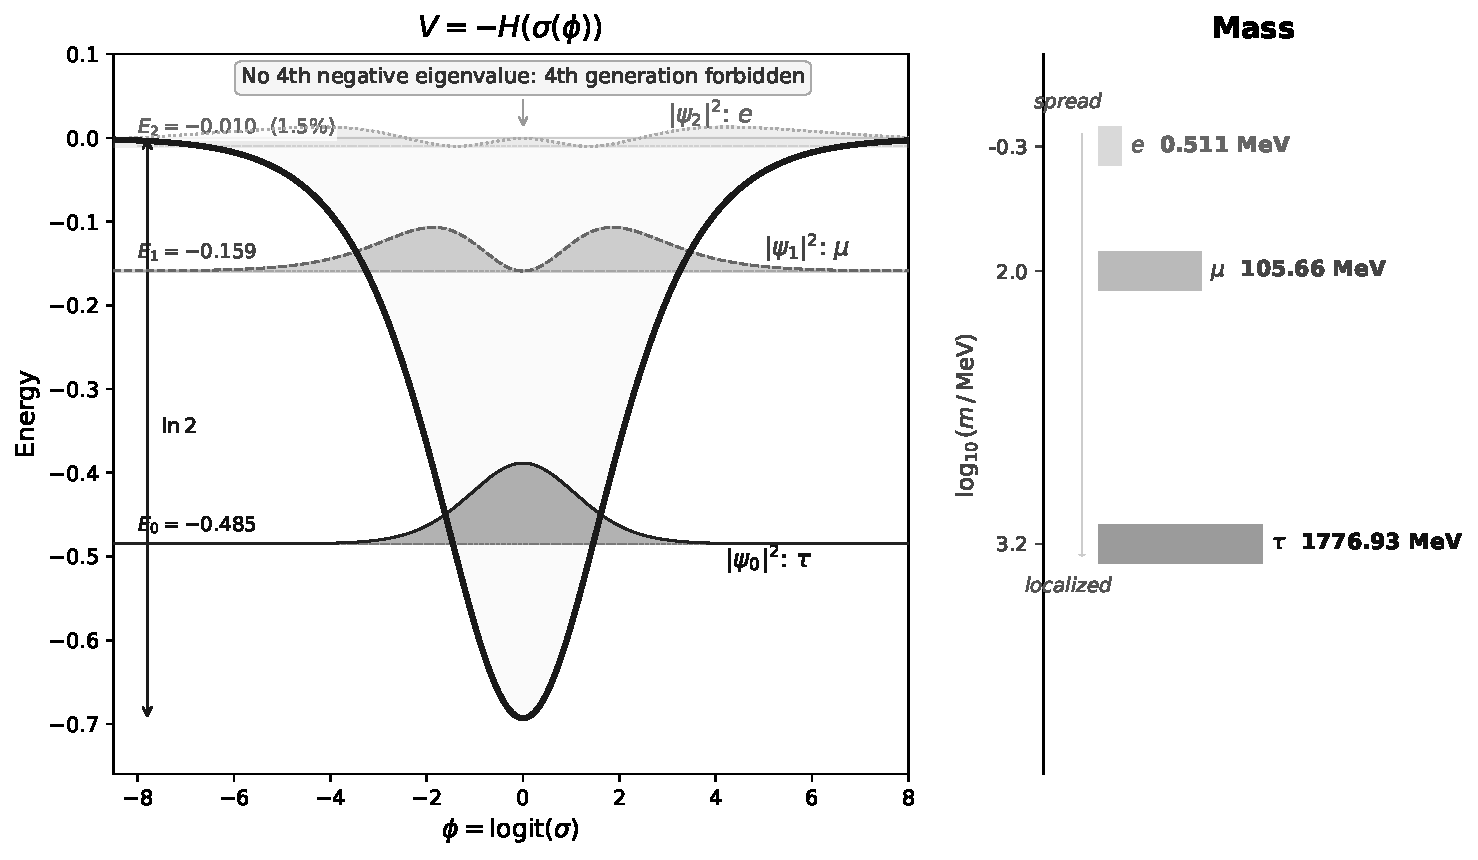
\includegraphics[width=\textwidth]{fig_potential.pdf}
\caption{ポテンシャル $V = -H(\sigma(\phi))$ とその3つの束縛状態の確率密度 $|\psi_n|^2$（左）。局在した状態ほど重い粒子に対応する（右）。第4の負固有値は存在しない：第4世代は存在できない。}
\label{fig:potential}
\end{figure}

この井戸に閉じ込められる準位の数を N
とする。井戸の中に何個の半波長が収まるかを半古典近似（WKB）で見積もる。整数個が収まるごとに1つの束縛状態が存在する：

\[n_\mathrm{WKB} = \frac{1}{\pi}\int_{-\infty}^{\infty}\sqrt{2H(\sigma(\phi))}\,d\phi = 2.781\]

Maslov 補正を含む標準規約では、第 $k$ 状態の閾値は $n_{\mathrm{WKB}}$ \textgreater{} $k - 1/2$ である。$n_{\mathrm{WKB}}$ = 2.781 は第3状態の閾値 2.5 を 0.281 上回る一方、第4状態の閾値 3.5 には 0.719 足りない。したがって WKB は N = 3 を示唆する。厳密な束縛状態数とこの半古典的作用カウントの差を ε = N − $n_{\mathrm{WKB}}$ = 3 − 2.781 = 0.219 と定義する\footnote{厳密な区間包含 0.219188 は Paper~II で与える。}。ε \textgreater{} 0 は第3状態がぎりぎり束縛されていることを反映する。「どれだけ限界的か」を測る数値は半古典規約の選択に依存し、Maslov 込みの規約で同じ隔たりを測れば 2.781 − 2.5 = 0.281 になる。本論文の展開量は一貫してこの $\varepsilon$ であり、§6–§8 で導く結合定数と混合角の NLO 補正を支配する。
N = 3 は、3つの要素---座標の選択、運動項の規格化、エントロピーの種類---からなる構成の帰結である。第一に、座標 φ = logit(\sigma) は、傾斜作用を線形化する座標としてアフィン変換を除いて一意であり、その目盛りは A1 の二値指示子が固定する（§2.4）。第二に、運動項の規格化は §2.4 の正準規格化 $g = 1$ である。第三に、Shannon エントロピーは強加法性（連鎖則）を含む Khinchin の公理系を満たす唯一のエントロピーである（Khinchin の定理~\cite{aczel,khinchin}）。この構成のもとで、N = 3 は区間演算により厳密に証明される（§3.2）。

\subsection{厳密証明}\label{ux53b3ux5bc6ux8a3cux660e}

\textbf{定理（N = 3）。} §2 のシュレーディンガー方程式はちょうど3つの束縛状態を持ち、その固有値は区間演算により厳密に包含されている：

\[
\begin{aligned}
E_0 &= -0.4850022531029642374452777658 \pm 10^{-24},\\
E_1 &= -0.1590522216188561779934190 \pm 10^{-24},\\
E_2 &= -0.010423393062109459327616 \pm 10^{-22}
\end{aligned}
\]

第4の負固有値は存在せず、本質スペクトルは 0 から始まる（有限グリッドの小さな正値は箱の離散化産物）。

\emph{証明（計算機支援・区間演算）。} パリティにより半直線 $[0,\infty)$ 上の Neumann 問題（偶）と Dirichlet 問題（奇）に分解する。ポテンシャルの単調性に基づく区間包含の下で Prüfer 角を区間伝播し、解析的テール評価と組み合わせて試験エネルギーでの Prüfer 角の厳密な上下界を得る。Sturm 振動理論により負固有値の個数は Prüfer 角の回転量で厳密に数えられ、偶セクターにちょうど2個、奇セクターにちょうど1個---合わせて N = 3---が従う。固有値包含は区間係数の検証済み高階 Taylor 積分器による両側シューティングで認証される。独立実装（Arb 球演算）が束縛状態数 N = 3 を再認証する。付属の検証コードは、sech 型（Pöschl--Teller 型~\cite{poschl}）試行関数3本の Rayleigh 商による変分上界でも、3つの負固有値の存在を独立に追認する。証明書コード3本を supplementary に同梱。□

\textbf{世代との対応。} この3つの束縛状態 $\psi_0, \psi_1, \psi_2$ は、フェルミオンの3世代に対応する。束縛エネルギーの順序 $|E_0| > |E_1| > |E_2|$ は波動関数の局在度の順序に対応する---最も深く束縛された $\psi_0$ は井戸の中心に最も局在し、限界的に束縛された $\psi_2$ は最も広がる。§8 で示すように、この局在度が質量に対応し、$\psi_0, \psi_1, \psi_2$ はそれぞれ最も重い世代から最も軽い世代（荷電レプトンでは τ, μ, e）に対応する。束縛状態の個数（3）とその順序構造が、世代の個数と質量階層に構造的に対応する。第4の負固有値が存在しないことは、第4世代が存在しないことを予測する。質量比と混合角の定量的な導出は §8 で示す。

\section{三つの空間次元}\label{ux3064ux306eux7a7aux9593ux6b21ux5143}

§3 で N = 3 が証明された。次の問いは：この3つの束縛状態の数学的構造が物理的構造に対応するなら、何次元の空間で実現可能か。以下でこれを検討する。

V = −H と同じ井戸型を d 次元空間の動径プロファイルとして考える。ここで $\sigma(r)$ は $\sigma(\phi)$（$\phi \in \mathbb{R}$）と同じ井戸型を動径変数 $r \geq 0$ に移したものである---定義域の違いは後述の全直線量子化との比較で扱う。d 次元シュレーディンガー方程式を標準的な偏波分解により1次元の動径方程式に帰着させると、追加の有効力 (d−1)(d−3)/(8r²) が現れる：

\[V_\mathrm{eff}(r) = -H(\sigma(r)) + \frac{(d-1)(d-3)}{8r^2}.\]

分子 (d−1)(d−3) は d = 1 と d = 3 でゼロになり、V = −H
がそのまま残る。その他の次元では、この幾何学的項が作用素を変形する：

\needspace{8\baselineskip}
\begin{longtable}[]{@{}lll@{}}
\toprule\noalign{}
d & (d-1)(d-3)/8 & 作用素への影響 \\
\midrule\noalign{}
\endhead
\bottomrule\noalign{}
\endlastfoot
1 & 0 & 変形なし \\
2 & -1/8 & 引力的な項が加わる（余分な状態を生む向き） \\
3 & \textbf{0} & \textbf{変形なし：井戸の形が保存} \\
4 & +3/8 & 斥力的な項が加わる（限界的な第3状態を失う向き） \\
≥5 & ≥1 & 強い斥力 \\
\end{longtable}

全直線量子化（$\phi \in \mathbb{R}$）は端点で本質的自己共役であり境界条件を要しない。A3（非存在は状態ではない---境界での追加データの禁止）\PII{}の下では、この全直線上の正準量子化を基準とし、空間的実現には正準作用素へ余分な逆二乗項を加えないことを要求する。この要求を満たすのは係数 $(d-1)(d-3)/8$ が消える $d = 1, 3$ のみである。なお、逆二乗項が零でも全直線問題と動径問題が同一になるわけではない---半直線の動径模型は原点の端点構造（自己共役拡張の選択）を追加した別模型であり、この対応の比較からは外れる（Paper~II）。

2つの実現整合条件が d = 1 を排除する。第一に、フェルミオン性（CAR）は A1--A3 から導かれる（基底独立二値性）\PII{}。その空間的実現が要する半整数スピンはスピン統計定理により d ≥ 3 で成立する（π₁(SO(d)) = Z₂ となり、有限次元スピノル表現を持つ二重被覆 Spin(d) が存在する）。第二に、スピン2場（重力）の実現---§9.1 と同じく前提として置き、その導出は後続論文で扱う---が動的に伝播するには d ≥ 3 が必要である（d ≤ 2 では Weyl テンソルが恒等的にゼロで局所的自由度がない）。

以上を定理としてまとめる。

\textbf{定理（d = 3）。} A3 による全直線量子化の選択の下で、d = 3 は以下を同時に満たす唯一の空間次元である：\emph{(i)} 井戸の作用素を余分な幾何学項なしに保つ：d = 1, 3；\emph{(ii)} スピン統計接続が成立：d ≥ 3；\emph{(iii)}
重力が伝播（Weyl テンソルが非自明）：d ≥ 3。交差：\{3\}。

\emph{証明。} (i) 遠心力項 (d−1)(d−3)/(8r²) = 0 は d = 1 または 3 のとき且つそのときに限る；(ii) π₁(SO(d)) = Z₂ は d ≥ 3；(iii) Weyl テンソルは時空次元 ≤ 3（すなわち空間 d ≤ 2）で恒等的にゼロ；伝播する重力には d ≥ 3 が必要。□



\section{射影平面からのゲージ構造}\label{ux5c04ux5f71ux5e73ux9762ux304bux3089ux306eux30b2ux30fcux30b8ux69cbux9020}

世代数 N = 3（§3）と空間次元 d =
3（§4）は独立に導出された---にもかかわらず同じ値 N = d = 3
を取る。この一致の上に、体 F₃ 上の3次元空間 F₃³ を構成する。本章では、そこから生じる幾何学的構造が、標準模型のゲージ構造と同じ数学的構成を持つことを示す。

\subsection{ゲージ構造の起源}\label{ux30b2ux30fcux30b8ux69cbux9020ux306eux8d77ux6e90}

$N = d = 3$ からどのようなゲージ構造が生じるか。鍵は、世代と色の根本的な違いにある。

クォークのカラー（赤・緑・青）は縮退している---どの色も同じエネルギーを持つため、優先的な基底がない。この等価性が連続的な回転対称性 $\mathrm{SU}(3)$ を生む。世代は違う。$V = -H$ の3つの束縛状態は全て異なるエネルギー（$E_0 \neq E_1 \neq E_2$、Sturm--Liouville の定理）を持つため、優先固有基底が存在する。この基底を保存する対称性は離散的であり、ゲージ対称性としては連続群を支えない\footnote{§8.1 の質量読み出しに現れる $2C_F$ は $N = 3$ の内部局在化 Casimir であり、これと両立する。}。

§3 で $N = 3$（束縛状態数）、§4 で $d = 3$（空間次元）が導出された。この一致から体 $\mathbb{F}_3 = \{0, 1, 2\}$ 上の3次元空間 $\mathbb{F}_3^3$ が定まる。以下の射影空間の構成には体（群ではなく）が必要であり、$N = 3$ が素数であるため $\mathbb{F}_3 = \mathbb{Z}/3\mathbb{Z}$ が $N$ 元素の唯一の体として一意に定まる。$\mathbb{F}_3^3$ の中から原点を除いた2次元の断面を見ると、$\mathbb{F}_3^2 = \{0,1,2\} \times \{0,1,2\}$---$3 \times 3$ のグリッド---が現れる。この9点が以降の構成の出発点となる。

$3 \times 3$ グリッド上で直線を引くと、同じ傾きの直線は平行になり交わらない。射影幾何ではこれらが「無限遠の1点」で合流する---透視図法で平行な線路が地平線上の1点に収束するのと同じ原理である。$\mathbb{F}_3^2$ 上の直線には4つの傾き（水平・垂直・右斜め・左斜め）があり、各傾きに対応する無限遠点が1つずつ生じる。この4点を結んだものが無限遠ライン $L$---地平線に相当する。

元の9点に4つの無限遠点を加えると $9 + 4 = 13$ 点。これが射影平面 $\mathrm{PG}(2, \mathbb{F}_3)$ である---$\mathbb{F}_3^3$ の原点を通る1次元部分空間を「点」、2次元部分空間を「ライン」と定義した空間で、13点・13ライン・各ライン上4点・各点を通るライン4本という対称的構造を持つ（図~\ref{fig:pg23}）。

\begin{figure}[t]
\centering
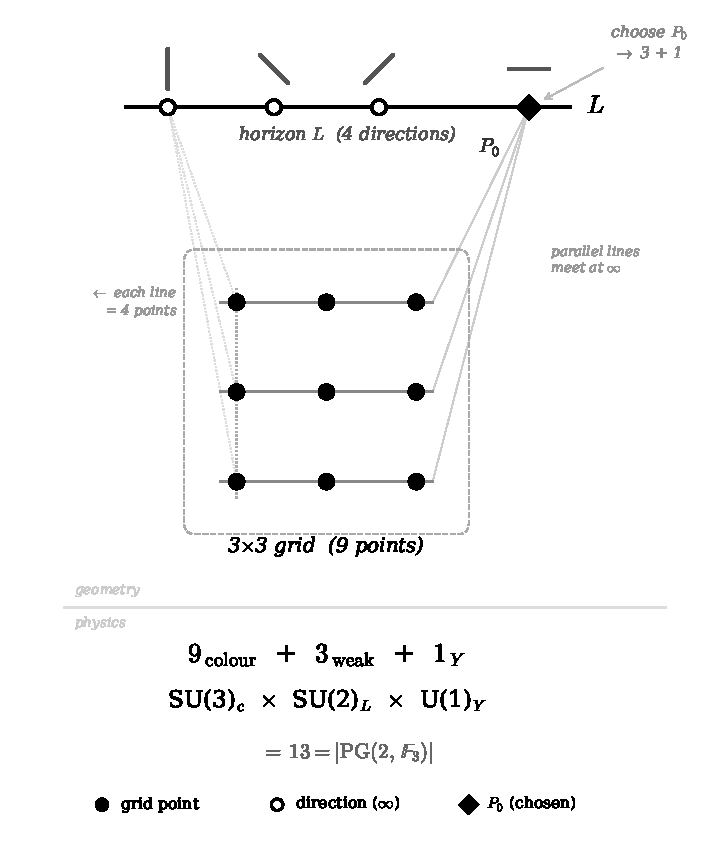
\includegraphics[width=0.75\columnwidth]{fig_pg23_v2.pdf}
\caption{射影平面 $\mathrm{PG}(2,\mathbb{F}_3)$ の構造。$3 \times 3$ グリッド（9点、黒丸）の平行線が無限遠ライン $L$ 上の方向（白丸）で合流する。$P_0$（黒菱形）を選ぶことで $9{+}3{+}1 = 13$ の分割が生じ、$\mathrm{SU}(3){\times}\mathrm{SU}(2){\times}\mathrm{U}(1)$ のセクター構造に対応する。}
\label{fig:pg23}
\end{figure}

$\mathrm{PG}(2, \mathbb{F}_3)$ の完全な対称性 $\mathrm{PGL}(3, \mathbb{F}_3)$ のもとでは、13点は全て等価であり分割は生じない。ここで無限遠ライン $L$ 上の4点のうち1つを基準点 $P_0$ として固定する---この組 $(P_0, L)$ を旗（フラグ）と呼ぶ。旗の固定は構成内の基準選択であり、$\mathrm{PGL}(3, \mathbb{F}_3)$ は旗に推移的に作用するため、どの旗を選んでも同型な分割を与える。固定により13点が3つのグループに分かれる：$L$ の外にある9点（$3 \times 3$ グリッド）、$L$ 上で $P_0$ 以外の3点、$P_0$ の1点。$P_0$ だけでは $1{+}12$ の2グループにしかならず、旗を選んで初めて $9{+}3{+}1$ の3グループが生じる。これが3つの力を区別する最小の構造である：

\[N^2_{(9\;\mathrm{colour})} + N_{(3\;\mathrm{weak})} + 1_{(1\;\mathrm{hyp})} = N^2 + N + 1.\]

$N = d$ を満たすのは $N = 3$ のみである（$N = 2, 4, 5$ はいずれも $d = 3 \neq N$）。$N = 3$ が素数であることは、$N$ 元の体が素体 $\mathbb F_3 = \mathbb Z/3\mathbb Z$ に一意に定まることを保証する。この一致から分割 $9{+}3{+}1$ の全ての数が $N$ のみで決まる：$N^2 = 9$、$N{+}1 = 4$（うち参照点を除き $N = 3$）、参照点 1。合計 $N^2{+}N{+}1 = 13$。52個のフラグ（点-ライン対）がラプラシアンの基底を与える（§6.3）。

\subsection{13点から標準模型ゲージ群へ}\label{ux70b9ux304bux3089ux6a19ux6e96ux6a21ux578bux30b2ux30fcux30b8ux7fa4ux3078}

この $9{+}3{+}1$ の分割が、標準模型のゲージ群 $\mathrm{SU}(3){\times}\mathrm{SU}(2){\times}\mathrm{U}(1)_Y$ のセクター構造と一致する。

\noindent\textbf{9点 $\to$ SU(3)。} $L$ 外の9点はアフィン平面 $\mathrm{AG}(2, \mathbb{F}_3)$ を構成する。この9点は $(a,b) \in \mathbb{F}_3^2$ でラベルされ、3次元内部表現における有限 Weyl 演算子 $W_{a,b} = X^a Z^b$ を自然に添字づける。単位元 $W_{0,0}$ は中心成分であり、残る8つの非自明な Weyl 成分が traceless セクターを構成する。この rank 2・dimension 8 のコンパクト単純リー完成は Killing--Cartan 分類により $\mathfrak{su}(3)$ に一意に定まる。9番目の中心成分は大域バリオン数 $\mathrm{U}(1)_B$ に対応する（ゲージ化されない大域荷であり、アノマリーフリーな厳密結合は $B{-}L$ である、§8.4）。

\noindent\textbf{3点 $\to$ SU(2)。} $L$ 上で $P_0$ 以外の3点は、基準点に対する3つの非自明な弱方向を与える。この3方向の最小非可換コンパクトリー完成は3生成子の $\mathfrak{su}(2)$ であり、その二重項表現が弱 SU(2) 作用を与える。

\noindent\textbf{1点 $\to$ U(1)$_Y$。} 基準点 $P_0$ はアーベル中心モジュール位相に対応し、物理的にはハイパーチャージ $\mathrm{U}(1)_Y$ に対応する。

\noindent\textbf{直積構造の保証。} アフィン平面の平行移動は無限遠ライン $L$ を固定する---グリッドをずらしても「方向」は変わらない。カラーセクター（9点）の変換は電弱セクター（$3{+}1$ 点）と混合しない。これは $\mathrm{PG}(2, \mathbb{F}_3)$ の入射構造から従う幾何学的性質であり、三つのセクターが互いに混合しないという直積型の構造を与える---標準模型のゲージ群と同じ形である。群の大域形（標準模型では $\mathbb{Z}_6$ 商を含む~\cite{baezhuerta}）は幾何だけでは決まらず、粒子担体への忠実作用から定まる（Paper~II）。

\[n^2{=}n \xrightarrow{V=-H} N{=}3 \xrightarrow{d=3} \mathbb{F}_3^3 \xrightarrow{\text{方向を数える}} 13\text{点} \xrightarrow{\text{旗}} 9{+}3{+}1 \xrightarrow{\text{Killing-Cartan}} \mathfrak{su}(3)\oplus\mathfrak{su}(2)\oplus\mathfrak{u}(1).\]

この数学的導出結果は、実験で確立されたゲージ構造 $\mathrm{SU}(3) \times \mathrm{SU}(2) \times \mathrm{U}(1)$ と一致する。

ライン上の4点は $\mathrm{SU}(2)$ 二重項の4つの実自由度---$\mathrm{SU}(2){\times}\mathrm{U}(1) \to \mathrm{U}(1)_\mathrm{em}$ の破れに必要な3つの Goldstone ボソンと物理的 Higgs---に対応する。$V = -H$ は $\phi = 0$（$\sigma = 1/2$）で最小値 $-\ln 2$ を取り、$\phi \to \pm\infty$ でゼロに戻る安定な井戸である（$V''(0) = 1/4 > 0$）。真空は場の消失点（$\sigma \in \{0,1\}$）ではなく内部点 $\sigma = 1/2$ に位置する---標準模型で負の二次項（$\mu^2 > 0$）が果たす役割、すなわち真空を対称点から有限の場の値へ移すことを、ここでは井戸の形状が担う。

\textbf{存在変数 $n$ の配位分解。} ゲージ構造は存在変数 $n$（§2）の内部空間に多様な配位を生む。$n$ 自体は唯一であるが---A3 により、区別する性質を持たない裸の存在は1つに帰着する---$\mathrm{PG}(2, \mathbb{F}_3)$ のゲージ構造が複数の内部配位を定義する。各配位 $i$ は世代（$V = -H$ の束縛状態）とゲージ量子数（PG 上の位置）で特徴づけられ、占有数 $n_i \in \{0,1\}$ を持つ。$n$ は1つ、$n_i$ は多数---唯一の存在が多様なフェルミオンとして発現する。配位分解は：

\[\sum_{i} \hat{n}_i = \hat{n}, \qquad \hat{n}_i^2 = \hat{n}_i, \qquad \hat{n}_i \hat{n}_j = \delta_{ij}\,\hat{n}_i\]

第一式は存在が配位に分解されること、第二式は二値性（n² = n）の継承、第三式は唯一の存在単位がちょうど一つの配位を占めること---一粒子状態空間の直交分解（$\hat n_i$ は互いに直交し $\hat n$ に足し上がる射影）---を述べる。この相互排他性は独立の仮定ではなく、存在の二値性（A1）と唯一性（A3）の帰結である。これは一粒子レベルの構造である。Pauli 排他律そのもの---同一モードの二重占有の禁止と交換反対称性---は、各配位をモードとする多体実現（CAR 構成）\PII{}が担い、そこでは異なる配位は同時に占有されうる。具体的な配位ラベルは §5.3 のフェルミオン表現で固定される。$n_i = 0$ は非存在を意味しない---存在が別の配位を占めていることを意味する。

\subsection{フェルミオンの多様性の起源}\label{sec:fermion-diversity}

§5.2 までで、PG(2, F₃) の13方向が標準模型のゲージ群と同じ形の構造を持つことを確立した。しかし13方向はフェルミオンそのものには対応しない。13方向はゲージ対称性---力の構造---を定め、フェルミオン構造はこのゲージ群の\textbf{表現}として現れる。ここでは、唯一の存在変数 $n$ がなぜ多様な物質粒子構造として発現するかを示す。

$n$ は唯一である。ゲージ構造が出現する前、$n$ は量子数を持たない---世代ラベルもカラーもアイソスピンもない裸の自由度である。区別する性質がなければ複数の $n$ は同一であり（Leibniz の不可弁別者同一の原理）、$n$ は唯一に留まる。$\mathrm{PG}(2, \mathbb{F}_3)$ のゲージ構造がこれを変える：ゲージ群の表現が内部空間に多様な「居場所」---配位---を生み、各配位に占有数 $n_i \in \{0,1\}$ が対応する。

各配位 $i$ は2つのラベルで特徴づけられる：世代 $k$（$V = -H$ のどの束縛状態か、$k = 1,2,3$）と、ゲージ表現 $\alpha$（$\mathrm{PG}(2, \mathbb{F}_3)$ のどのセクターに属するか）。すなわち $n_i = n_{k,\alpha}$ である。ゲージ群 $\mathrm{SU}(3){\times}\mathrm{SU}(2){\times}\mathrm{U}(1)$ の表現が1世代あたり16状態を与える。左右非対称性（$\mathrm{SU}(2)$ が左巻き場のみに作用すること）は、この粒子種指定の一部であり、本論文では導出しない。Paper~II では、明示した列挙条件の下で混合配置が排除され、左右の割り当ては大域的な向きの規約を除いて一意に定まる。下表のハイパーチャージは、$9{+}3{+}1$ セクター構造、湯川閉包、$\nu_R$ の包含、および局所可換ゲージ因子を1つとする指定（$B{-}L$ はゲージ化されない大域荷、§5.2）と両立する唯一の anomaly-free 割当であり、その演算子レベルの導出も同論文で与えられる：

\vspace*{0.55\baselineskip}
\begin{center}
\small
\renewcommand{\arraystretch}{1.15}
\begin{tabular}{@{}l@{\qquad}l@{\qquad}l@{}}
\toprule
表現 & 内容 & 状態数 \\
\midrule
$(\mathbf{3}, \mathbf{2}, 1/6)$ & 左巻きクォーク $Q_L$ & 6 \\
$(\mathbf{3}, \mathbf{1}, 2/3)$ & 右巻き上型 $u_R$ & 3 \\
$(\mathbf{3}, \mathbf{1}, {-}1/3)$ & 右巻き下型 $d_R$ & 3 \\
$(\mathbf{1}, \mathbf{2}, {-}1/2)$ & 左巻きレプトン $L_L$ & 2 \\
$(\mathbf{1}, \mathbf{1}, {-}1)$ & 右巻き荷電レプトン $e_R$ & 1 \\
$(\mathbf{1}, \mathbf{1}, 0)$ & 右巻きニュートリノ $\nu_R$ & 1 \\
\bottomrule
\end{tabular}
\end{center}
\vspace*{0.35\baselineskip}

\noindent 合計 $16 \times 3$ 世代 $= 48$ 配位。$\nu_R$ の包含は湯川閉包および $B{-}L$ 保護された Dirac 型ニュートリノ構造（§8.4）に必要である。これは上で定義した配位分解の具体化であり、添字 $i$ が世代ラベル $k$ とゲージ表現ラベル $\alpha$ の組 $(k,\alpha)$ を走ることを意味する。各配位が継承する二値性 $n_i^2 = n_i$ が、多体実現では各モードの占有を $\{0,1\}$ に制限する---これが Pauli 排他律の占有数表現である~\cite{pauli}。異なる配位の相互排他性は、唯一の存在単位がどの配位を占めるかという一粒子レベルの構造である（§5.2）。ゲージ群 $\mathrm{SU}(3){\times}\mathrm{SU}(2){\times}\mathrm{U}(1)$ の生成子は $8{+}3{+}1 = 12$ 個のゲージボソン（グルーオン8、$W^+W^-Z$ 3、光子1）に対応する。これに §5.2 のヒッグス粒子1を加え、48フェルミオン・12ゲージボソン・1ヒッグスが標準模型の全粒子内容を構成する。

こうして、唯一の存在（$n$）から多様な物質（$n_i$）が生まれる。鍵は $\mathrm{PG}(2, \mathbb{F}_3)$ のゲージ構造が「区別可能な居場所」を生み出すことにある---ゲージ対称性がなければ存在は無特徴のまま一つに留まり、ゲージ対称性があるからこそ48種のフェルミオンが現れる。物質の多様性はゲージ構造の帰結である。

この構成の内部整合性は、固有関数の参加比 $D_{PR} = (\int\rho\,d\phi)^2/\int\rho^2\,d\phi$（$\rho = \sum_n \psi_n^2$ は3束縛状態の合計密度）$= 13.06 \approx |\mathrm{PG}|$（検証コードで再現可能）と、52$\times$52 フラグラプラシアンのスペクトル分解により独立に確認される\footnote{Paper~II の有限核定理とスペクトルゲージ分解の系。}。導出のいかなるステップにも自由パラメータは含まれない。この構成の正当性は、§6--§10 で導かれる独立な物理量が全て 0.0006\%--2.6\% の精度で実験と一致することにより裏付けられる。

\section{ゲージ結合定数}\label{sec:couplings}

§5.2 でゲージ群と対応する構造（どの力が存在するか）が導かれた。本章ではその強さ（結合定数）を導く。

\subsection{Weinberg 角}\label{weinberg-ux89d2}

§5.2 の分割 9+3+1
が結合定数に対応する値を与える。弱セクターの3方向が13方向に占める割合が Weinberg
角 \cite{weinberg}（弱混合角） $\sin^2\!\theta_W$ である。点の重みは旗を固定する前の対称性が定める：PGL(3, F₃) は PG(2,3)
に推移的に作用するため、13方向は等しい重み（不変測度）を持つ。旗の固定はこの重みを変えず、13点を 9+3+1 に分類するだけである。Weinberg 角は、弱3方向が全13方向に占める分率として読む---分母に全内部方向を取る選択の指定である：

\[\sin²θ_W = 3/13 = 0.2308 \quad (\text{実験: } 0.23122\;\overline{\mathrm{MS}}\text{、}M_Z\text{ で},\; 0.2\%)\]

ツリーレベル予測 3/13 = 0.23077 と \(\overline{\mathrm{MS}}\)
スキームの実験値 0.23122 ± 0.00003 \cite{pdg} との 0.2\%
の偏差は1ループ輻射補正と整合的である。これがツリーレベルで W/Z
質量比を与える：$m_W/m_Z$ = $\cos\theta_W$ = √(10/13) = 0.8771（実験: 0.8813, 0.5\%；偏差は輻射補正と整合的）。

\subsection{強結合定数}\label{ux5f37ux7d50ux5408ux5b9aux6570}

強結合定数は、弱セクターの分率をカラーセクターのランクで分配して決まる。カラーセクターの9方向のうち独立な方向は
rank(SU(3)) = 2 個（Cartan 生成子）であり、$\sin^2\!\theta_W$
をこの2方向へ等分配する読み出しを取ると：$\alpha_s^{(0)}$ = $\sin^2\!\theta_W$ / (N−1) = 3/26 = 0.1154（この分配則は選択の指定である）。§3
のスペクトル的限界性 ε = 0.219 が NLO 補正を与える。補正は N²+1 = 10 個の非弱
PG 方向（カラー9 + ハイパーチャージ1）を通じて分配される：

\[α_s = (3/26)(1 + ε/(N²+1)) = 0.1179 \quad (\text{実験: } 0.1179\;\overline{\mathrm{MS}}\text{、}M_Z\text{ で},\; 0.01\%)\]

k = N²+1 = 10 の値は PG(2, F₃) の非弱方向の数から従う。NLO 補正は本論文を通じて $1 \pm \ell\varepsilon/k$ の形をとり、分母 k は補正が分配される有限支持のサイズである---非弱セクター（$\alpha_s$）は k = N²+1 = 10（アフィン＋ハイパーチャージ）、世代混合（$\sin\theta_C$）は k = N² = 9（アフィン平面）、全 PG モード（$m_H/v$・sin²θ₂₃）は k =
\textbar PG\textbar{} = 13（全射影空間）、弱3方向（sin²θ₁₃）は k = N = 3。符号と係数 ℓ を含む (ℓ, k) の観測量ごとの割り当ては選択の指定である。

\subsection{微細構造定数}\label{ux5faeux7d30ux69cbux9020ux5b9aux6570}

Weinberg 角と強結合定数は PG(2,3)
上の点の比率だけで決まった。微細構造定数はそれでは足りない---内部空間の全スペクトル構造が必要である。

電磁結合定数の逆数 1/α は、電磁相互作用の弱さを測る。観測される電荷は物質場によって遮蔽された電荷であり、遮蔽が強いほど結合は弱く、1/α は大きい。本枠組みでは 1/α は、裸の光子の伝播コスト λ₁ と物質場の遮蔽量 Z の和として（自己無撞着補正 $-\alpha$ を除いて）定まり、Thomson 点の値は遮蔽項が支配する。4次元 QED
ではこの構造が Dyson
方程式として定式化される。0次元でも同じ構造が成り立つが、伝播子が定数になるため頂点補正と自己エネルギーが同じレゾルベントで決まり、4次元の摂動的相殺 $Z_1 = Z_2$ が厳密な代数的恒等式として成立する（証明は Paper~II）。自己無撞着方程式は：

\[\frac{1}{\alpha} + \alpha = \lambda_1 + Z\]

となる。右辺の λ₁ は裸の光子逆伝播子（伝播コスト）、Z はスカラーチャネルスペクトル量（遮蔽量）に対応する。この対応はスペクトル的なものである：$Z$ はレゾルベントトレースで、そのエネルギー分母構造が物質真空偏極と一致する。方程式の形（左辺 $1/\alpha + \alpha$ と係数1）は、入射電流を Thomson 点の電磁電流に対応させる指定に属する。self-consistent な予言としての完全な正当化と、この指定の下で物理根が一意に定まることの証明は、いずれも同論文で与えられる。なお $Z$ は $1/|E_2| = 95.94$ に支配されるが、$E_2$ は §3.2 の区間演算で厳密に認証されており、この感度は不確かさを生まない。

ゲージ場が内部空間を伝播する際の最小コスト λ₁
は、内部空間上のラプラシアンの最小非ゼロ固有値で決まる。ゲージ相互作用は位置（点）と方向（ライン）の両方を含むため、拡散の対象はフラグ（点-ライン対）である。PG(2,
F₃) の52個のフラグを頂点とするグラフラプラシアン $\mathcal{L}$ のスペクトルは：

\needspace{12\baselineskip}
\begin{longtable}[]{@{}lll@{}}
\toprule\noalign{}
固有値 & N = 3 での値 & 多重度 \\
\midrule\noalign{}
\endhead
\bottomrule\noalign{}
\endlastfoot
0 & 0 & 1 \\
(N+1) − √N & 2.268 & 12 \\
(N+1) + √N & 5.732 & 12 \\
2(N+1) & 8 & 27 \\
\end{longtable}

最小非ゼロ固有値 λ₁ = 4 − √3 = 2.268 が、1/α の対応式（§6.3）で裸の光子逆伝播子に対応する量である。λ₁
\textgreater{} 0
は閉じ込めの描像と整合する---正のスペクトルギャップは、カラー荷を持つ状態が漸近的に自由伝播しないことに対応する。

遮蔽項 $Z$ は、3世代の物質場によるスカラーチャネルスペクトル量に対応し、内部運動演算子のレゾルベントで決まる。内部運動演算子は、世代セクター（$K_\mathrm{gen}$、固有値は束縛エネルギー
\textbar $E_n$\textbar）とゲージセクター（$\mathcal{L}$、固有値
$\lambda_k$）のテンソル和である：

\[K_\mathrm{int} = K_\mathrm{gen} \otimes \mathbf{1} + \mathbf{1} \otimes \mathcal{L}\]

この形---テンソル和であること、および両因子を同一単位で測る相対スケール1---は、単一時計の単位条項の下で一意性定理として確立される\PII{}（積結合・ねじれ積・相対スケールの取り替えは排除される）。レゾルベントのトレースを各多重度で分解すると：

\[Z = \mathrm{Tr}[1/K_\mathrm{int}] = \zeta_V(1) + 12\,S_1 + 12\,S_2 + 27\,S_3 = 134.77613\]

ここで $\zeta_V$(1) = $\Sigma_n$ \textbar $E_n$\textbar⁻¹、$S_i$ = $\Sigma_n$
(\textbar $E_n$\textbar{} + $\lambda_i$)⁻¹。中間値は：$\zeta_V(1) = 104.28714$（$E_2^{-1} = 95.94$ が支配的）、$12S_1 = 14.57025$、$12S_2 = 6.05684$、$27S_3 = 9.86190$。27次元セクター（多重度 27 =
3³）の寄与 9.86 ≈ N² であり、QCD 真空偏極補正に対応するスペクトル構造を与える（付属の検証コードで全中間値を再現可能）。

λ₁ = 4 − √3 = 2.26795 と Z = 134.77613 を自己無撞着方程式に代入すると\footnote{実験の推奨値は $1/\alpha = 137.035999177(21)$（CODATA 2022）。本文の 137.0368 は先頭項であり、補正級数込みの高精度評価は Paper~II で扱う。}：

\[\frac{1}{\alpha} = \frac{(Z + \lambda_1) + \sqrt{(Z + \lambda_1)^2 - 4}}{2} = 137.0368 \quad (\text{実験: } 137.036,\; 0.0006\%)\]

\section{ヒッグスセクターと電弱対称性の破れ}\label{sec:higgs}

§6 でゲージ結合定数を導いた。標準模型にはもう1つ、スカラーセクターの自由パラメータがある---Higgs 自己結合 $\lambda$ である。本章ではこれに対応する数学的構造を導くとともに、真空の内部点固定と内部ポテンシャルの有界性（不安定性チャンネルなし）を示す。

\subsection{対称性の破れと Higgs 質量}

電弱対称性の破れとは、力学法則は対称なまま、真空（基底状態）が対称点から外れることである。$W$ と $Z$ が質量を持ち光子が質量を持たない以上、真空は場の消失点（対称点）にはあり得ない---破れは実験が要求する。標準模型はこれを Higgs ポテンシャル $V = -\mu^2|\Phi|^2 + \lambda|\Phi|^4$ の $\mu^2 > 0$ という仮定で実現する：原点を不安定化し、場を有限の値へ転がす。しかし「なぜ $\mu^2 > 0$ なのか」は標準模型の中では説明されない。

本論文の $V = -H(\sigma(\phi))$ は、この問いに構造で答える。2値 Shannon エントロピー $H$ は両端 $\sigma \in \{0,1\}$（場の消失点に対応する自明な配位）でゼロ、内部点 $\sigma = 1/2$ で最大であるから、$V = -H$ は端点で 0、内部点で最小値 $-\ln 2$ を取る安定な井戸である（$V''(0) = 1/4 > 0$）。さらに A2（$\sigma \neq 1$）と A3（$\sigma \neq 0$）は端点そのものを禁じる。したがって基底状態は必然的に内部点に座る---真空が対称点に座れないこと、すなわち破れの条件が、原点の不安定化ではなくエントロピーの形と公理から従う。真空の位置は $V$ の形の帰結であり、追加の仮定を必要としない。ヒッグス質量の読み出しは、この最小点における正の曲率 $V''(0) = 1/4$ を用いる。

§5.2で示したように、PG(2, F₃) のライン構造が Higgs の SU(2) 二重項に対応する。その中心での曲率が Higgs 質量を与える：$V''(0) = g_F(0) = \sigma(0)(1{-}\sigma(0)) = 1/4$（$\sigma = 1/2$ での Fisher 計量）。
\[m_H/v = \sqrt{V''(0)} = 1/2 \quad (\mathrm{LO})\]
NLO 補正はラプラシアン行列 $\mathcal{L}$ の全 $|\mathrm{PG}|$ = 13 モードから入る：
\[m_H/v = \frac{1}{2}\sqrt{1 + 2\varepsilon/|\mathrm{PG}|} = 0.5084 \quad (\text{実験: } 0.5082, 0.03\%)\]
これは $\lambda = (m_H/v)^2/2 = 0.1292$（実験：0.1291、0.06\%）に対応する。

\subsection{真空安定性と階層性問題}

標準模型の Higgs ポテンシャル $V_\mathrm{SM} = -\mu^2 h^2 + \lambda h^4$ は $h \to \infty$ で発散し、紫外補正 $\delta\mu^2 \propto \Lambda^2$ が電弱スケールとプランクスケールの間に $\sim 10^{34}$ の微調整を要求する（階層性問題）。さらに Higgs の四次結合 $\lambda(\mu)$ がくりこみ群により走り、$\mu \sim 10^{10}$\,GeV で負に転じるため、電弱真空は宇宙論的に準安定である。

$V = -H$ の内部セクターでは、これらの問題に対応する不安定性は生じない。$V = -H$ は有界（$|V| \leq \ln 2$）であり、高エネルギーでの発散がない。井戸の深さ $|V_{\min}| = \ln 2$ と曲率 $V''(0) = 1/4$ はともに $O(1)$ の代数的定数であり、その比 $|V_{\min}|/V''(0) = 4\ln 2 \approx 2.77$ は内部量どうしの比であり、微調整を要しない $O(1)$ の値である（4D の $v^2/\Lambda^2$ との対応は再構成マッチングを要する）。内部ポテンシャル $V = -H$ は有界である：$V \in [-\ln 2, 0]$。この有界性を 4D の走る結合 $\lambda(\mu)$ が負に転じないことの根拠と解釈するには、再構成マッチングを要する（完全な 4D 真空安定性の解釈、および高温での対称性回復など熱的性質との対応も同様）\PII{}。$V$ の形状は公理から固定されており、スケール依存性は $V$ の代数的構造を変えない。

さらに、$V = -H$ は $n \in \{0,1\}$ の正準自由エネルギーとして一意に定まる（§2）。PFE の最小演算子代数では第二の基本スカラーポテンシャルは生成されず、最小再構成は単一の Higgs 二重項を予測する。

\subsection{輻射補正と結合定数のまとめ}

\textbf{輻射補正との整合性。} 上記の予測は代数的値であり、$M_Z$ スケールの実験値との比較には走る量への 4D の RG 発展とループ補正を要する（§9.3）。弱角の次補正は本枠組みの読み出しから閉形式で定まる：$\Delta_\mathrm{rad} = \alpha\cdot 5N^3\!/|\mathrm{PG}|^3 = \alpha\cdot 135/2197 = 0.00045$（N と \textbar PG\textbar{} は本論文の量；係数 5 を含む指定された読み出しの下での導出は同論文）。これにより $\sin^2\!\theta_W = 3/13 + \Delta_\mathrm{rad} = 0.23077 + 0.00045 = 0.23122$ となり、$\overline{\mathrm{MS}}$ 実験値 $0.23122 \pm 0.00003$~\cite{pdg} と誤差の範囲で一致する。同様に $m_W/m_Z = \sqrt{10/13} = 0.8771$（先導）は実験値より $0.5\%$ 低い。この残差は標準模型のトップクォーク $\Delta\rho$ 補正と同程度の大きさと符号を持つが、$\Delta\rho$ を加えた比較は繰り込み方式の対応付けを要する条件付き計算である。

\textbf{まとめ。} $\sin^2\!\theta_W(M_Z) = 0.23122$（$<0.01\%$）、$\alpha_s(M_Z) = 0.1179$（0.01\%）、$1/\alpha_\mathrm{em} = 137.0368$（0.0006\%）、$m_H/v = 0.5084$（0.03\%）。4つの結合定数が全て $V = -H$ と PG(2,3) から導かれ、実験と一致する。真空は内部点に固定され、内部ポテンシャルは有界（不安定性チャンネルなし）であり、Higgs は1つだけである。4D の真空安定性・階層性問題との対応は再構成マッチングを要する命題である。

\section{フェルミオンの質量と混合}\label{ux30d5ux30a7ux30ebux30dfux30aaux30f3ux306eux8ceaux91cfux3068ux6df7ux5408}

§5--7 でゲージ構造、結合定数、ヒッグス質量に対応する構造を確立した。§3 で確定した3つの束縛状態と荷電レプトン3世代の対応に基づき、本章では束縛状態の局在度から質量比と混合角の数式を導く。導かれた値は、荷電レプトン・クォーク・ニュートリノの質量比および CKM/PMNS 混合角と高い精度で一致する。

\subsection{質量公式}\label{ux8ceaux91cfux516cux5f0f}

$V = -H$ の3つの束縛状態は局在度が異なる。最も深い $\psi_0$ は井戸の底に局在しゲージ場と最も強く結合するため、最も重い $\tau$ に対応する：

\begin{longtable}[]{@{}lllll@{}}
\toprule\noalign{}
束縛状態 & エネルギー & 局在度 & 対応粒子 & 質量 (MeV) \\
\midrule\noalign{}
\endhead
\bottomrule\noalign{}
\endlastfoot
ψ₀ & E₀ = −0.485 & 高（井戸の底） & τ & 1777 \\
ψ₁ & E₁ = −0.159 & 中 & μ & 106 \\
ψ₂ & E₂ = −0.010 & 低（井戸の縁） & e & 0.511 \\
\end{longtable}

質量比は波動関数の局在度で決まり、独立パラメータではない。鍵となる量は $R = \ln(m_\tau/m_e)/\ln(m_\mu/m_e)$ であり、3体の質量階層を1つの数に圧縮する。

\[V = -H \xrightarrow{\text{§3}} \psi_n \xrightarrow{\text{IPR}} \text{局在度} \xrightarrow{2C_F} m_n \xrightarrow{} R = 1.5293\]

各固有状態は束縛エネルギー \textbar $E_n$\textbar{}
と局在度を持つ。局在度は逆参加比 $\mathrm{IPR}_n$ = ∫\textbar $\psi_n$\textbar⁴dφ
で測られる。ゲージ場との結合強度は相互作用点における波動関数の振幅に比例する。内部空間で局在した状態ほど、その点での振幅が大きく、ゲージ場を介して大きな質量を獲得する。質量は局在度のべき乗に比例する：$m_n$ ∝ $\mathrm{IPR}_n^{\,b}$。本節の読み出しでは、指数 b を N = 3 セクターに付随する連続 $\mathrm{SU}(3)$ リフトの内部局在化 Casimir に取る：b = $2C_F$ = (N²−1)/N = 8/3\footnote{これはレプトンの物理的カラー荷ではなく、$N = 3$ の内部局在化 Casimir である。クォークでは同じ $N = 3$ 構造がカラーと一致する。Paper II \cite{paper2} 参照。}。

V = −H
の非調和性から小さな補正が生じる。各モードが井戸を異なる仕方でサンプルし、ビリアル比
$|\langle V\rangle_n|/T_n$（ポテンシャルエネルギーと運動エネルギーの比）がこれを測る。補正の指数はスペクトル
ζ 関数を通じて現れる限界性パラメータで決まる：半古典的作用カウント $n_{\mathrm{WKB}}$ = 2.781 は、厳密な束縛状態数 N = 3 に ε = 0.219
だけ足りず、モードあたりの限界性は δ = ε/N = 0.073。

完全な質量公式は：

\[m_n \propto |E_n| \times \mathrm{IPR}_n^{2C_F} \times (|\langle V \rangle_n| / T_n)^{\varepsilon/N}\]

3つの因子は異なる起源を持つ：

\needspace{12\baselineskip}
\begin{longtable}[]{@{}lll@{}}
\toprule\noalign{}
因子 & 物理的意味 & 決定要因 \\
\midrule\noalign{}
\endhead
\bottomrule\noalign{}
\endlastfoot
\textbar $E_n$\textbar{} & エネルギースケール & 束縛エネルギー \\
IPR\^{}\{$2C_F$\} & 局在度 → 結合強度 & 群論（Casimir） \\
(|⟨V⟩|/T)\^{}\{ε/N\} & 非調和補正 & スペクトル的限界性 \\
\end{longtable}

全指数が V = −H から決まる。結果：

\[R = \frac{\ln(m_\tau/m_e)}{\ln(m_\mu/m_e)} = 1.5293 \quad (\text{実験: } 1.5294,\; 0.006\%)\]

（全スペクトル量は $|\phi|_{\mathrm{max}}$ = 100, Δφ = 1.25×10⁻⁴ ($N_{\mathrm{grid}}$ =
1600001) で計算し、グリッド解像度の倍増および箱サイズの拡大で安定であることを検証済み。）

本節の読み出しは、群論的 Casimir $b = 2C_F = 8/3$ を先に固定する。この固定された値を質量公式に代入すると、独立に Koide \cite{koide} の $Q \approx 3/2$（本論文の規約は $Q = (\sum\sqrt{m})^2/\sum m$。標準的な規約 $\sum m/(\sum\sqrt{m})^2 = 2/3$ の逆数）とスペクトル条件 $c = \varepsilon/N$ が同時に満たされる。したがって Koide は $b$ を決める入力ではなく、$b = 8/3$ の出力検証である：

\needspace{12\baselineskip}
\begin{longtable}[]{@{}lll@{}}
\toprule\noalign{}
b & c (Q=3/2) & 偏差 \\
\midrule\noalign{}
\endhead
\bottomrule\noalign{}
\endlastfoot
2.0 & 0.437 & 500\% \\
2.5 & 0.163 & 120\% \\
\textbf{8/3 = $2C_F$} & \textbf{0.0730} & \textbf{0.07\%} \\
2.78 & 0.012 & 84\% \\
3.0 & -0.107 & 246\% \\
\end{longtable}

\needspace{12\baselineskip}
\begin{longtable}[]{@{}llll@{}}
\toprule\noalign{}
& 予測 & 実験 & 精度 \\
\midrule\noalign{}
\endhead
\bottomrule\noalign{}
\endlastfoot
$m_\tau/m_e$ & 3481 & 3477 & 0.1\% \\
$m_\mu/m_e$ & 207.0 & 206.8 & 0.1\% \\
R & 1.5293 & 1.5294 & 0.006\% \\
Q (Koide) & 1.499985 & 1.50001(2) & 2σ（PDG 質量より算出） \\
\end{longtable}

3つのレプトン質量は独立パラメータではなく、1つの井戸の3つのモードであり、指数 $2C_F$ = 8/3 は本節の読み出しが定める。0次元ではループ積分が存在しないため、異常次元を動的に生成する走りが存在しない。有限群の Peter-Weyl 定理により、群上の熱核は有限和 K(t) = $\Sigma_\rho$ dim(ρ) $\chi_\rho$(g) $e^{-\lambda_{\rho} t}$ となり、べき乗則を含まない---指数減衰のみが許容される。したがって指数は表現が定める量であり、その値として連続 SU(3) リフトの内部局在化 Casimir $2C_F$ を取るのが本節の読み出しである\footnote{この読み出しの一意性は Paper~II~\cite{paper2} で扱われる：質量応答の関数形は一意性定理として証明され、指数の割り当ては明示した読み出しの指定として扱われる。}。R = 1.5293 の 0.006\% 一致は、束縛状態とレプトン世代の対応を定量的に支持する。Koide 関係が輻射補正の下で安定であることは Sumino~\cite{sumino} が論じている。

\subsection{クォーク質量}\label{ux30afux30a9ux30fcux30afux8ceaux91cf}

§8.1 の質量公式はレプトンで R = 1.5293
を再現した。同じ公式がクォークにも適用できるか。公式そのものは変わらない---変わるのは井戸の深さだけである。

レプトンはカラー一重項（色を持たない）であり、ポテンシャルは V = −H
の1本分である。クォークは3色を持つ。カラー三重項の井戸は、三つの同型な色寄与を共通の存在座標 $\phi$ 上で足し合わせ、$V = -3H$ と取る---これも選択の指定である。井戸が3倍深くなるため、束縛状態の数も増える---V = −3H
は5個の束縛状態を支える（$n_{\mathrm{WKB}}$ = 4.82）。以下の表では井戸の深さ倍率（$V = -\kappa H$ の $\kappa$）を $\kappa$ と書く：

\needspace{8\baselineskip}
\begin{longtable}[]{@{}lllll@{}}
\toprule\noalign{}
セクター & 作用素 & $\kappa$ & 束縛状態 & 使用モード \\
\midrule\noalign{}
\endhead
\bottomrule\noalign{}
\endlastfoot
レプトン & −H & 1 & 3 & (0,1,2) = τ,μ,e \\
アップ型 & −3H & 3 & 5 & (1,2,3) = t,c,u \\
ダウン型 & −3H（運動項に補正） & 3 & 4 & (0,1,2) = b,s,d \\
\end{longtable}

\noindent\textbf{アップ型。} モード 0 は深く閉じ込められ $I_3 = -1/2$ セクターに属する。アップ型クォーク（$I_3 = +1/2$）はモード (1,2,3) を使い、同じ質量公式から $R_\mathrm{up} = 1.777$（実験: 1.770, 0.4\%）。

\noindent\textbf{ダウン型。} アップ型とダウン型は同じ SU(2) ダブレットに属し、同じ $V = -3H$ を感じるが、弱アイソスピンの符号が異なる（$I_3 = +1/2$ vs $-1/2$）。この符号が質量公式に補正を与える。

SU(2) ダブレット (u, d) の全ゲージ荷の和 $2C_F + 1/N_c = N_c$ は厳密な代数的恒等式である。この補正の物理的機構は PG(2, $\mathbb{F}_3$) の幾何に由来する。ライン $L$ 上の $N+1 = 4$ 点のうち、基準点 $P_0$ が二重項の向き付け（どちらを $I_3 = +1/2$ と呼ぶか）を定める基準であり、残る3点が SU(2) ゲージ変換を生成する。$I_3$ の符号反転はこの向き付けの反転に対応し、内部空間上での SU(2) 作用の向きを反転させる。この反転が、全荷 $N_c$ を§2.2 の Bernoulli Fisher 計量 $g_F(\phi) = \sigma(1{-}\sigma) = \operatorname{Var}(n)$（その一意性が \v{C}encov の定理 \cite{cencov}）に負符号で結合させる。有効質量は：

\[m_\mathrm{eff}(\phi) = 1 - N_c \sigma(1{-}\sigma)\]

これはダウンセクター読み出しの静的 Fisher 極限形である。実際に解く演算子は位置依存質量の対称形 $-\tfrac{1}{2}\,\partial_\phi\,(1/m_\mathrm{eff})\,\partial_\phi - 3H$ である（付属コードの離散化と同一）。補正係数 $g_c = -N_c = -3$（第2.4節の規格化 $g$ とは別の量）は SU(2) ダブレットの代数的構造から定まる。補正後の演算子は負固有値を4個持ち（$-1.5709, -0.5455, -0.1952, -0.00733$；箱サイズ $L_\mathrm{box} = 40/80/120$ で安定）、そのうち3モード (0,1,2) が物理窓 b, s, d に対応する---どのモードを物理窓に取るかはアップ型と同様に読み出しの指定である（窓はセクターごとに異なる：レプトンは3モード全部、アップ型は (1,2,3)、ダウン型は (0,1,2)）。モード (0,1,2) で $R_\mathrm{down} = 2.273$（実験: 2.276, 0.1\%）。

3つの荷電フェルミオンセクターの質量比が全て再現される：

\needspace{12\baselineskip}
\begin{longtable}[]{@{}llllll@{}}
\toprule\noalign{}
セクター & $\kappa$ & $g_c$ & R（予測） & R（実験） & 精度 \\
\midrule\noalign{}
\endhead
\bottomrule\noalign{}
\endlastfoot
レプトン & 1 & 0 & 1.529 & 1.529 & 0.006\% \\
アップ & $N_c$ = 3 & 0 & 1.777 & 1.770 & 0.4\% \\
ダウン & $N_c$ = 3 & −$N_c$ & 2.273 & 2.276 & 0.1\% \\
\end{longtable}

\noindent ここで R は対数階層の形を捉えるものであり---質量比を一様に伸縮しても（各 $m_i/m_j$ を共通の冪に上げても）不変である---個別の質量ではない。表の精度列は予測値の実験中心値に対する偏差である。実験側の R には軽クォーク質量の不確かさ（PDG 2026: $m_u = 2.16 \pm 0.07$ MeV 等）が約 ±0.15--0.25\% の幅として伝播し、比較はさらに各質量のスキーム・スケール規約（軽クォークは 2 GeV の MS-bar、c・b は $m(m)$、t は直接測定質量）に依存する。どのモードがどのクォークに対応するかの割り当ては物理的な指定（5モードのうちどの3つか）であって導出ではない\footnote{個別クォーク質量の大きさは Paper~II で条件付きに扱う。}。

\subsection{CKM 混合}\label{ckm-ux6df7ux5408}

§8.1--8.2 で質量比が確定した。次に世代間の混合 \cite{km} を導く。なぜ
$V_{ub}$ は小さく、Cabibbo
角~\cite{cabibbo}はあの値なのか。標準模型はこれらを説明しない。V = −H
では、ポテンシャルの対称性が前者に、第3世代の限界性が後者に対応する。

ポテンシャル $V = -H$ は対称である：$V(\phi) = V(-\phi)$。これにより固有関数はパリティが確定する：$\psi_0$ 偶、$\psi_1$ 奇、$\psi_2$ 偶。異なるモードの直接的重なりは Sturm-Liouville 直交性により $\langle\psi_0|\psi_2\rangle = 0$。$\psi_0$ と $\psi_2$ はともに偶であるから、V-パリティ奇の混合演算子 $M$ に対して $\langle\psi_0|M|\psi_2\rangle = 0$---先導的な $0 \leftrightarrow 2$ 遷移が禁じられる：

\[V_{ub}\big|_\mathrm{tree} = 0\]

観測値 $|V_{ub}| \approx 0.004$ は Wolfenstein 階層の高次から生じる。V-パリティにより tree/direct 項は厳密に零であり、遠隔世代遷移は少なくとも $O(\varepsilon^3)$ まで抑制される。Paper~II の読み出しでは、最初の非零項は $2\varepsilon^4$ である（下記参照）。

Cabibbo 角はスペクトル的限界性から従う。第3束縛状態 $\psi_2$ は限界的に束縛されている---その束縛エネルギー $|E_2| = 0.010$ は井戸の深さのわずか1.5\%である。この限界性を測る量は、厳密な束縛状態数と半古典的作用カウントの差である：

\[\varepsilon = N - n_\mathrm{WKB} = 3 - 2.781 = 0.219\]

混合角は質量固有状態と弱固有状態の不一致を反映する。第3束縛状態が限界的（$\varepsilon > 0$）であることが混合の源であり、$\varepsilon \to 0$ でこの源が除去されると、3世代は保たれたままフレーバー遷移が消える。混合角を $\varepsilon$ の級数として与える読み出し---遷移を運ぶ演算子と、その次数・分母---は観測量ごとの選択の指定である（§6.2 の一覧）。2次まで：

\[\sin\theta_C = \varepsilon(1 + \varepsilon/N^2) = 0.2245 \quad (\text{実験: } 0.2243,\; 0.10\%)\]

この値は無遮蔽の内部値である。色遮蔽を合成した観測読み出しは $\sin\theta_C \cdot (1-x) = 0.22435$（$x = N^2\alpha/(2\pi|\mathrm{PG}|) = 9\alpha/(26\pi)$ は色遮蔽の展開量；導出は同論文）。

Cabibbo 角の値は、第3世代がかろうじて存在するという事実---世代セクターのスペクトル量 ε = 0.219（§3.1 で V = −H のみから定義され、全ての混合読み出しに共通に入る）---の直接的な表現である。もし第3束縛状態がもう少し深く束縛されていれば（ε → 0）、世代間の混合は消失し、全てのフレーバー遷移は禁止される。

Cabibbo 角から Wolfenstein 階層 \cite{wolfenstein} が従う：$|V_{us}| \sim \varepsilon$、$|V_{cb}| \sim \varepsilon^2$、$|V_{ub}|$ は少なくとも $O(\varepsilon^3)$ まで抑制され最初の非零項は $2\varepsilon^4$（実験値: 0.225, 0.041, 0.004）。NLO 補正は $1 \pm \ell\varepsilon/k$ の形をとる。分母 $k$ と符号・係数 $\ell$ の割り当ては §6.2 の一覧のとおり（$\sin\theta_C$ は $1+\varepsilon/9$、$\sin^2\theta_{13}$ は $1-2\varepsilon/3$）。

$V(\phi) = V(-\phi)$ というパリティ対称性は直接の $0\leftrightarrow2$ フレーバー遷移を抑制するが、QCD 真空角を単独では固定しない。パリティだけでは $\theta\in\{0,\pi\}$ が残る。

観測可能な strong-CP 角は $\bar{\theta} = \theta_\mathrm{QCD} + \arg\det M_q$ である。Paper~II の strong-CP matching 定理は、生成作用語・正則化 fermion determinant line・大ゲージ loop の実現まで A1--A3 を保って適用すると $\arg\det(M_uM_d) = 0$ と裸の $\theta_\mathrm{QCD} = 0$ がともに従い、したがって minimal PFE reconstruction の matching 点で $\bar\theta(\mu_0) = 0$ となることを示す。ここで裸の QCD 角を消すのは、正の測度 ray を保存するユニタリスカラーが $\{1\}$ に限られること（Paper~II の順序付き測度線の自明性）であって、本節の V-パリティ単独ではない。またこれは matching 点での言明であり、全 scale の厳密零ではない---弱 CKM ループと threshold を含む $\bar\theta_\mathrm{IR}$ は Paper~II でも未評価である。したがって、PQ 型大域 U(1) の不在から排除される PQ 型アクシオンを超えて、アクシオン様粒子一般の不存在を主張することはできない。しかし CKM セクターでは CP 破れが観測されている（$J = 3.08 \times 10^{-5}$）。これは裸の $\theta_\mathrm{QCD} = 0$ と矛盾しない：CKM 位相は $\varepsilon$ の高次で生じ（$J = \pi\varepsilon^5/N_\mathrm{flags}$、$N_\mathrm{flags} = 52$ は旗の総数（§5.1）---同論文で指定する読み出しの下の定理）、matching 点の条件は厳密にゼロのままである。

フレーバーと strong-CP の結果をまとめる：

\medskip
\begin{center}
\small
\begin{tabular}{@{}p{0.24\linewidth}p{0.40\linewidth}p{0.30\linewidth}@{}}
\toprule
量 & 予測 & 実験 \\
\midrule
$V_{ub}$（ツリー） & 0（最初の非零項は $2\varepsilon^4$、Paper~II） & $|V_{ub}| = 0.004$（高次で生成） \\
裸の $\theta_\mathrm{QCD}$ & \textbf{V-パリティの帰結ではない}（matching 点の値 $\bar\theta(\mu_0)=0$；Paper~II の測度線自明性と strong-CP matching 定理） & $\bar\theta < 10^{-10}$ \\
CKM CP 破れ & $J = \pi\varepsilon^5/N_\mathrm{flags}$（Paper~II の読み出しの下の定理） & $3.06 \times 10^{-5}$（実験 $3.08 \times 10^{-5}$） \\
\bottomrule
\end{tabular}
\end{center}
\bigskip

\subsection{ニュートリノ}\label{ux30cbux30e5ux30fcux30c8ux30eaux30ce}

§8.1--8.3 で荷電フェルミオン（レプトン、クォーク）の質量比と混合角を導いた。残るはニュートリノである。

\textbf{質量予測。}
ニュートリノはカラー一重項であるため $\kappa = 1$ で $V = -H$ に結合する---荷電レプトンと同じポテンシャルである。質量比 $R$ は井戸の形状（IPR とビリアル比）のみに依存し、粒子種には依存しない。同じ井戸は同じ $R$ を与える。$R_\nu = R_\mathrm{lepton} = 1.529$ が従う---これが本節の、実験入力を含まない予測である。正常順序と振動データ~\cite{nufit}（$\Delta m^2_{21} = 7.537 \times 10^{-5}~\mathrm{eV}^2$、$\Delta m^2_{31} = 2.521 \times 10^{-3}~\mathrm{eV}^2$）を条件として、この比が絶対質量を定める\footnote{$\pm 0.03$\,meV の不確実性は振動データ入力からの伝播であり、理論に自由パラメータはない。正常順序は本節では入力条件であり、その独立導出は定理として与えられる\PII{}（$R_\nu > 1$ と $(m_3/m_2)^2 = 169/5 > 1$ の帰結）。}：

\needspace{12\baselineskip}
\begin{longtable}[]{@{}lll@{}}
\toprule\noalign{}
量 & 予測 & 状態 \\
\midrule\noalign{}
\endhead
\bottomrule\noalign{}
\endlastfoot
$m_1$ & 0.32 ± 0.03 meV & 未測定 \\
$m_2$ & 8.69 meV & 整合 \\
$m_3$ & 50.2 meV & 整合 \\
$\Sigma m_i$ & 59.2 ± 0.3 meV & Planck 以下（\textless120） \\
\end{longtable}

フラグラプラシアンのスペクトルが exact に固定するのは $m_3/m_2 = |\mathrm{PG}|/\sqrt{N{+}2} = 13/\sqrt{5}$、すなわち $(m_3/m_2)^2 = 169/5$ である。質量二乗差比は、これと $R_\nu = R_\mathrm{lepton}$ から $t = m_1/m_2$ を消去した master 関係式 $\Delta m^2_{31}/\Delta m^2_{21} = (169/5 - t^2)/(1 - t^2) = 33.842\ldots$（表示 33.84）で与えられる\PII{}。非零の $m_1$ の下では 169/5 は質量二乗差比の exact 値ではない。本節が入力した $\Delta m^2$ の比自体は $2.521/0.07537 = 33.45$ であり、master 関係式は振動データの入力なしに 33.84 を与える。この 1.2\% は理論値と現在の測定値の差である。上表の絶対質量は入力側の比に基づく条件付き値であるため、master 関係式側を用いると $m_3$ と $\Sigma m_\nu$ は約 0.6\% 上振れする（$m_3/m_2 = 13/\sqrt5 = 5.814$ に対し上表は 5.777）。

この予測は反証可能である：本節の条件付き計算自体は質量順序を検定しないが、$\Sigma m_i > 70$\,meV は緊張を生む。$\Sigma m_i = 59.2$\,meV は正常順序の一般的な最小値（$m_1 \to 0$ で $58.89$\,meV）に近いため、CMB-S4~\cite{cmbs4}（$\sigma \sim 15$\,meV）がこの値付近を検出しても正常順序の確認にはなるが、本枠組みを一般的な最小シナリオと区別しない。枠組み固有の鋭いニュートリノ予言は比 $\Delta m^2_{31}/\Delta m^2_{21} = 33.8$ であり、JUNO が 2026--27 に検定する。

\noindent\textbf{混合角。}

§8.3 で CKM 混合角は $\varepsilon = 0.219$ から得られた---小さな値（$\sin\theta_C \approx 0.22$）である。ところがニュートリノの PMNS 混合角は大きい（$\sin^2\theta_{12} \approx 1/3$）。同じ $V = -H$ からなぜ大小2種類の混合が生じるのか。

答えは色荷の有無にある。クォークは色を持ち $V = -3H$ の深い井戸内にあるため、モードの重なりが小さい摂動的領域に入る---混合はこのため小さく、その展開径数は世代セクターの限界性 $\varepsilon$（§3.1）である。一方ニュートリノは色中性であり、PG(2,3) 上のゲージ方向の幾何的配分が混合角に対応する値を直接与える。

太陽混合角は1つの完全な電弱ライン（N+1 = 4 点）が PG
の13方向に占める分率：

\[\sin²θ_{12} = 4/13 = 0.3077 \quad (\text{実験: } 0.3088,\; 0.4\%)\]

大気混合角の LO は、純弱の N 方向と基準点を通る別の直線（N+1 点）との非交和が PG の13方向に占める分率 7/13 である。これに PG スケールの NLO 補正（k
= \textbar PG\textbar{} = 13）が加わると：

\[\sin²θ_{23} = (7/13)(1 + ε/13) = 0.5475 \quad (\text{第二オクタント})\]

LO の分率 7/13 は 1/2
を上回るため、第二オクタントを予測する。NuFIT 6.1 \cite{nufit} の global best fit は第一オクタント（sin²θ₂₃ = 0.470）に移ったが、オクタントは未確定であり、予測値 0.5475 は 3σ 許容域（0.432--0.587）の内側にある---第二オクタントの検定は DUNE / Hyper-Kamiokande に委ねられる。第二オクタント側の値 0.561 に対する偏差は 2.4\%（約 1σ、実験精度 \textasciitilde2.5\% に対して）である。特に断らない限り、本論文で引用する NuFIT 6.1 の値は、上記の Δm² 入力と整合する SK-atm なし・正常順序のデータセットである。反応器角は $\sin^2\!\theta_{13}$ = 1/(N·\textbar PG\textbar) = 1/39 に NLO
補正（k = N = 3）を加えて：

\[\sin²θ_{13} = (1/39)(1 - 2ε/3) = 0.0219 \quad (\text{実験: } 0.02249,\; 2.6\%)\]

3つの PMNS 混合角の予測と実験値をまとめる：

\vspace*{0.55\baselineskip}
\begin{center}
\small
\renewcommand{\arraystretch}{1.08}
\begin{tabular}{@{}lllll@{}}
\toprule
角度 & LO & NLO 予測 & 実験 & 精度 \\
\midrule
sin²θ₁₂ & 4/13 = 0.308 & --- & 0.3088 & 0.4\% \\
sin²θ₂₃ & 7/13 = 0.538 & 0.5475 & 0.561（第二オクタント局所値） & 2.4\% \\
sin²θ₁₃ & 1/39 = 0.026 & 0.0219 & 0.02249 & 2.6\% \\
\bottomrule
\end{tabular}
\end{center}
\vspace*{0.35\baselineskip}

和則：7/13 = 3/13 + 4/13（LO で sin²θ₂₃ = $\sin^2\!\theta_W$ + sin²θ₁₂）は、13 を分母とする有限計数の恒等式である。ただしこれは形式的な和であり、純弱の3点は完全電弱ラインの4点に含まれる（両集合は交わり、合併は4点）ため点集合の分割ではない---大気角の7方向の幾何的由来は上記の非交和である。NLO 補正はこの和則を破り、Paper~II が反証可能な予言として与える。

\noindent\textbf{Dirac 粒子。}
\label{ux30cbux30e5ux30fcux30c8ux30eaux30ceux306f-dirac-ux7c92ux5b50}

ニュートリノは Dirac か Majorana か---未解決の実験的問題である。本枠組みは明確な予測を与える。構成に現れる全てのフェルミオン演算子は数演算子 $\hat{n}$（ベルヌーイ族の十分統計量）の関数であり、位相回転 $a \to e^{i\theta}a$ の下で不変である：アノマリーフリーな組み合わせ $\mathrm{U}(1)_{B-L}$ は厳密であり、マヨラナ双線形 $aa + a^\dagger a^\dagger$（$\Delta(B{-}L) = 2$）はこの演算子代数の外にある。V-パリティは $\nu$ と $\nu^c$（レプトン数 $L = \pm 1$）を Dirac フェルミオンに対にする（演算子レベルの証明：Paper~II~\cite{paper2} の Dirac 選択定理）。

従ってニュートリノなし二重ベータ崩壊は厳密にゼロである：

\[0\nu\beta\beta = 0 \quad (\text{nEXO \cite{nexo}〜2030 で検証可能})\]

以上で、フェルミオンの質量比、混合角、ニュートリノの性質が V = −H と PG(2, F₃) の構造から得られた（絶対質量は正常順序と振動データを条件とする）。標準模型がこれらを独立な自由パラメータとして扱うのに対し、本枠組みでは全てが1つの方程式 $V = -H$ の代数的展開の異なる側面である。

\section{時空への接続}\label{ux6642ux7a7aux3078ux306eux63a5ux7d9a}

§2--8 の全ての計算は内部空間（φ
座標）で行われた。空間も時間も登場しない。それでは、この0次元の理論はどのようにして4次元の時空と接続するのか。本章ではこれを3段階で示す：時空の次元とシグネチャ (3,1)（§9.1）、内部空間と時空の独立性（§9.2）、そして0次元の代数的値が4次元の実験値に対応する理由（§9.3）。

\subsection{時空次元と重力}\label{ux6642ux7a7aux6b21ux5143ux3068ux91cdux529b}

§4 で空間次元 $d_{\mathrm{space}}$ = 3
を導出した。しかし「なぜ4次元時空か」は別の問いである---時間が1次元であることは自明ではない。以下では2つの独立な経路が同じ D = 4 を与えることを示す---いずれも前提を置いた整合性検査である（以後、空間次元を d、時空次元を D = d + 1 と書き分ける）。

第一の経路は重力の自由度から来る。D 次元時空における質量ゼロのスピン2粒子（重力子）は D(D−3)/2 個の物理的自由度を持つ（Poincaré 群の表現論から従い、特定の D を仮定せず、Einstein 方程式も前提としない）。一方、V = −H の N = 3 束縛状態は N−1 = 2 個の独立な内部自由度を与える（3つの確率が1に和するため）。Poincaré 対称性・スピン2場・ゲージ簡約を前提とする整合性検査として、時空の力学的自由度（重力子の偏極）を内部自由度と一対一に対応させると：

\[D(D−3)/2 = N − 1 = 2 \quad \Longrightarrow \quad D = 4\]

第二の経路は射影幾何から来る。射影平面 PG(2, ℂ) = ℂP² は実4次元多様体であり、N = 3 に対して：

\[D = \dim_\mathbb{R}(\mathbb{C}P^{N-1}) = 2(N-1) = 4\]

2つの経路をまとめる：

\needspace{12\baselineskip}
\begin{longtable}[]{@{}llll@{}}
\toprule\noalign{}
経路 & 入力 & 等式 & 結果 \\
\midrule\noalign{}
\endhead
\bottomrule\noalign{}
\endlastfoot
重力子の自由度 & スピン2の偏極数 & D(D−3)/2 = N−1 = 2 & D = 4 \\
射影幾何の担体 & 複素担体 ℂP² & $\dim_{\mathbb R}$(ℂP\^{}\{N−1\}) = 2(N−1) & D = 4 \\
\end{longtable}

両方が整合するのは N = 3 のみである。

この2つの経路は独立である---一方は場の理論の表現論（スピン2偏極）、他方は純粋な代数幾何（複素担体 ℂP²）に基づく。同じ D = 4 が独立な論理から従うことは、N = 3 の内部整合性を示す非自明なチェックである。

D = 4 が定まっても、シグネチャは (4,0)、(3,1)、(2,2) のいずれかでありうる。有限体 $\mathbb{F}_3$（N = 3 の素数性から）と複素担体 $\mathbb{C}^3$（ユニタリ実現から）は、同じ N = 3 に係留された独立な構成である（標数が異なるため体の準同型 $\mathbb{F}_3 \to \mathbb{C}$ は存在せず、$\mathbb{F}_9$ を経由する持ち上げも成立しない）。両者を結ぶのは Heisenberg--Weyl 系の指数ラベル（$\mathbb{F}_3$ 側）と表現担体（$\mathbb{C}^3$ 側）の対応であり、保存されるのは Weyl 交換関係と MUB 構造である。$\mathbb{C}^3$ は複素構造を最初から備えている。さらに、§2.2 で A2 が開いた内部座標 $\phi$ の転送作用 $S = \int[\tfrac{1}{2}\dot{\phi}^2 + V]\,d\tau$ が1つの発展パラメータ $\tau$ を持つため、4つの実方向のうち1つが発展方向として区別される。複素構造と単一の発展方向だけではシグネチャは一意に定まらない。(3,1) の選択は、$M_2(\mathbb{C})_{sa}$ 上の行列式形式と $\mathrm{SL}_2(\mathbb{C}) \to \mathrm{SO}^+(1,3)$ の構造への接続として定まる。シグネチャは (3,1) に固定される。

4次元では Lovelock の定理 \cite{lovelock}
が重力場方程式を一意に定める：2階以下の微分方程式は Einstein 方程式
\[G_{\mu\nu} + \Lambda g_{\mu\nu} = \kappa T_{\mu\nu}\]
のみである。Jacobson \cite{jacobson}
は因果的地平線上の δQ = $T_H$ dS
から同じ方程式が従うことを示した。本理論のエントロピーは S = H(P)
であるから、Lovelock（幾何的）と
Jacobson（熱力学的）の両経路が二値エントロピーから Einstein 重力に至る。

\subsection{なぜ内部空間と時空は独立か}\label{ux306aux305cux5185ux90e8ux7a7aux9593ux3068ux6642ux7a7aux306fux72ecux7acbux304b}

座標 φ = logit(\sigma) は内部空間に、座標 x
は時空に住む。なぜ両者は独立なのか。

答えは $V = -H$ の構成にある。$V = -H(\sigma(\phi))$ は Bernoulli 自由度の内部ゼロモードとして構成されたポテンシャルであり、明示的な時空座標 $x$ を含まない。しかし $\partial V/\partial x = 0$ というポテンシャルの非依存性だけでは、混合した運動項を排除できない。分解を成立させるのは、$\phi$（内部）と $x$（時空）を独立な自由度とし、生成子が別々の因子に作用して交差項を持たないという構成である。このとき全ハミルトニアンは $\hat{H} = \hat{H}_\phi + \hat{H}_x$ の形を取り、Hilbert 空間は $\mathcal{H}_\mathrm{int}(\phi) \otimes \mathcal{H}_\mathrm{space}(x)$ とテンソル積に分解される。

この合成空間は dim ≥ 3 であるから（$\mathcal{H}_\mathrm{int}(\phi)$ は世代因子だけで3次元、$\mathcal{H}_\mathrm{space}(x)$
は無限次元）、Gleason の定理 \cite{gleason} が §2 の検出確率 $\sigma = \langle n \rangle$
を標準的な Born
則に一意に拡張する---測定規則は公理ではなく、テンソル積構造の帰結である。

2つの観測的事実がこれを裏付ける。第一に、全ゲージ結合は世代に依存しない---φ
と x が結合していないことの直接的な証拠である。第二に、0D
理論は無次元量（質量比、混合角）のみを計算し、有次元量（絶対質量）は時空を要する---これはテンソル積構造の予測そのものである。

スピンとの類似がこの構造を照らす。スピン代数は有限次元であり Lagrangian
に依存しないが、4次元の物理量（磁気モーメント、微細構造）を決定する。世代も同じである---V
= −H という有限次元の構造が、4次元の質量比と混合角に対応する。

\subsection{0D 値と 4D 実験値の対応原理}\label{sec:correspondence}

テンソル積構造は、0D の代数的値がなぜ 4D のくりこみ済み理論のツリーレベル値と一致するかを説明する。0D の値は代数的定数である。4D では、ツリーレベルとはループ補正がゼロの極限---すなわち時空の力学が内部構造に影響しない極限---であり、これはまさにテンソル積 $\mathcal{H}_\mathrm{int}(\phi) \otimes \mathcal{H}_\mathrm{space}(x)$ が保証する独立性に対応する。輻射補正は時空因子 $\mathcal{H}_\mathrm{space}$ に由来するループ運動量の効果であり、内部因子 $H_\mathrm{int}$ の代数的値にサブパーセントの補正として加わる（§7、$\sin^2\theta_W = 3/13 + \Delta_\mathrm{rad} = 0.23122$）。0D の値は RG 固定点でも UV 境界条件でもなく、4D 理論との比較の基準点となる代数的に決定された唯一の点である---走る量には 4D の RG 発展とループ補正が加わり、離散的な状態数などは走らない。

以上により、内部構造（φ）と時空（x）の関係が確立された。V = −H が質量比、混合角、結合定数に対応する内部値を与える。時空因子は全体のエネルギースケールに加え、走る量への 4D の RG 発展とループ補正を供給する。

\clearpage
\section{結果}\label{ux7d50ux679c}

以上から、1つの方程式 V = −H と1つの幾何構造 PG(2, F₃)
から、標準模型の構造と一致する数学的構造が得られ、かつ標準模型の物理定数20個と 0.0006\%--2.6\% の精度で一致する計算結果が、調整可能パラメータなしに得られることを示した。さらに6個（$|V_{cb}|$, $|V_{ub}|$, $\delta_\mathrm{CKM}$, $\delta_\mathrm{PMNS}$, $m_3/m_2$, $\Delta m^2_{31}/\Delta m^2_{21}$）は、指定された演算子語による読み出しとフラグラプラシアンのスペクトル構造を必要とし、導出される\PII{}。なお、標準模型の26個のうち唯一の有次元パラメータである電弱スケール v は 0D では定まらず（§9.2）、その決定は再構成マッチングを要する---本論文の予測はすべて v を単位に取った無次元量（および Δm² を条件とする §8.4 の絶対質量）である。以下に結果の一覧を示す（実験値は PDG 2026~\cite{pdg}、NuFIT 6.1~\cite{nufit}、CODATA 2022~\cite{codata} による）。最大偏差の2行（sin²θ₂₃ 2.4\%・sin²θ₁₃ 2.6\%）は、当該量の実験不確かさに対していずれも約 1σ の内側にある（§8.4）。ただし sin²θ₂₃ の比較は第二オクタント局所値 0.561 に対するものであり、NuFIT 6.1 の global best fit は第一オクタント（0.470）にある---オクタントは未確定で、予測値は 3σ 許容域の内側にある（§8.4）。

\needspace{15\baselineskip}
\bigskip
\begin{center}\textbf{Table 1.} 標準模型定数との対比。\end{center}
\nopagebreak[4]\smallskip\nopagebreak[4]
\begin{center}\footnotesize
\begin{tabular}{@{}lcccc@{}}
\toprule
パラメータ & 予測値 & 実験値 & 精度 & \S \\
\midrule
\textbf{ゲージ結合定数} & & & & \\
$1/\alpha_\mathrm{em}$ ($\to g_1$)（Thomson 点） & 137.0368 & 137.036 & 0.0006\% & 6.3 \\
$\alpha_s$ ($\to g_3$)（MS-bar, $M_Z$） & 0.1179 & 0.1179 & 0.01\% & 6.2 \\
$\sin^2\!\theta_W$ ($\to g_1/g_2$)（MS-bar, $M_Z$） & $3/13$ & 0.23122 & 0.2\% & 6.1 \\
\textbf{Higgs} & & & & \\
$m_H/v$ ($\to\lambda$) & 0.5084 & 0.5082 & 0.03\% & 7 \\
\textbf{フェルミオン質量} & & & & \\
$R_\mathrm{lepton}$ ($\to y_e, y_\mu, y_\tau$) & 1.5293 & 1.5294 & 0.006\% & 8.1 \\
$R_\nu$ ($\to \nu$ 質量比；実験入力なし） & 1.529 & ---（未測定） & $R_\nu = R_\mathrm{lepton}$ & 8.4 \\
$R_\mathrm{up}$ ($\to y_u, y_c, y_t$) & 1.777 & 1.770 & 0.4\% & 8.2 \\
$R_\mathrm{down}$ ($\to y_d, y_s, y_b$) & 2.273 & 2.276 & 0.1\% & 8.2 \\
\textbf{CKM 混合} & & & & \\
$\sin\theta_C$ ($\to$ CKM $\theta_{12}$) & 0.2245 & 0.2243 & 0.10\% & 8.3 \\
\textbf{PMNS 混合} & & & & \\
$\sin^2\!\theta_{12}$ & $4/13$ & 0.3088 & 0.4\% & 8.4 \\
$\sin^2\!\theta_{23}$ & 0.5475 & 0.561（第二オクタント局所値） & 2.4\% & 8.4 \\
$\sin^2\!\theta_{13}$ & 0.0219 & 0.02249 & 2.6\% & 8.4 \\
\textbf{ニュートリノ質量} & & & & \\
$m_1$ ($\to \nu$ 絶対質量) & 0.32~meV & --- & 条件付き予測 & 8.4 \\
\textbf{強い CP} & & & & \\
$\bar\theta(\mu_0)$（matching 点） & 0（Paper II） & $\bar\theta < 10^{-10}$ & --- & 8.3 \\
\bottomrule
\end{tabular}
\end{center}

\needspace{15\baselineskip}
\bigskip
\begin{center}\textbf{Table 2.} その他の結果。\end{center}
\nopagebreak[4]\smallskip\nopagebreak[4]
\begin{center}\footnotesize
\begin{tabular}{@{}llcc@{}}
\toprule
物理量 & 導出 & 実験 & \S \\
\midrule
$N$（世代数） & $n_\mathrm{WKB} = 2.781 \to 3$ & 3 & 3 \\
$d$（空間次元） & $\{1,3\}\cap\{\geq 3\}\cap\{\geq 3\}$ & 3 & 4 \\
$D$（時空次元） & $D(D{-}3)/2 = N{-}1 = 2$ & 4 & 9.1 \\
シグネチャ & $M_2(\mathbb{C})_{sa}$ の構造への接続 & $(3,1)$ & 9.1 \\
ゲージ群 & $9{+}3{+}1$ (Killing--Cartan) & $\mathrm{SU}(3){\times}\mathrm{SU}(2){\times}\mathrm{U}(1)$ & 5 \\
ゲージ分解のスペクトル的検証 & 制限ラプラシアンのスペクトル $9{+}4{=}13$ & --- & Paper~II \\
第4世代 & 第4の負固有値なし & 排除済 & 3.2 \\
ニュートリノの性質 & $\mathrm{U}(1)_{B-L}$（$\hat{n}$構造）+ $V$-パリティ & --- & 8.4 \\
$m_W/m_Z$（先導） & $\sqrt{10/13} = 0.8771$ & 0.8813 (0.5\%) & 6.1; 7 \\
$Q$ (Koide) & 1.499985 & 1.50001 & 8.1 \\
$\sin^2\!\theta_W$（$3/13 + \alpha\cdot 135/2197$） & 0.23122 & 0.23122 ($<0.01\%$) & 7 \\
\bottomrule
\end{tabular}
\end{center}

\needspace{12\baselineskip}
\bigskip
\begin{center}\textbf{Table 3.} 検証可能な予測。\end{center}
\nopagebreak[4]\smallskip\nopagebreak[4]
\begin{center}\footnotesize
\begin{tabular}{@{}lp{0.36\linewidth}ll@{}}
\toprule
予測 & 値 & 検証実験 & \S \\
\midrule
$\Delta m^2_{31}/\Delta m^2_{21}$ & master 関係式（先導 $m_3/m_2 = 13/\sqrt{5}$、非零 $m_1$ 込み）= 33.84 & JUNO~\cite{juno}（2026--27） & Paper~II \\
$\theta_{23}$ オクタント & 第二（$>45^\circ$） & DUNE / HK（$\sim$2030） & 8.4 \\
$\delta_\mathrm{PMNS}$ & $197.1^\circ$ & DUNE / HK（$\sim$2030） & Paper~II \\
$\Sigma m_\nu$ & 59.2~meV（$\Delta m^2$ 入力の条件付き；$\approx$ 正常順序最小 58.9） & CMB-S4~\cite{cmbs4}（$\sim$2030） & 8.4 \\
$0\nu\beta\beta$ & 厳密にゼロ & nEXO~\cite{nexo}（$\sim$2030） & 8.4 \\
Koide 偏差 $\delta$ & $-1.5 \times 10^{-5}$ & Belle~II~\cite{belleii}（2027--30） & 8.1 \\
BSM 粒子 & なし & LHC / FCC & 3; 5.3 \\
\bottomrule
\end{tabular}
\end{center}

\bigskip

標準模型はこれらの物理量を、それぞれ独立に測定して入力すべきパラメータとして扱うが、本論文の導出過程に自由パラメータはない。§3 の束縛エネルギーは区間演算で認証され、§6.3 のラプラシアン固有値は閉形式で厳密である---有限グリッドに依存するのは局在度（IPR）・ビリアル比・参加比などの汎関数のみである。独立な複数の量にわたる一致は、この構成の妥当性を強く示している。本論文の全数値結果（Table 1–3 の全値と §3 の区間認証を含む）は、補足資料として添付する検証コード一式により独立に再現できる。

\section{結論}\label{ux7d50ux8ad6}

本論文は、標準模型で通常は独立な入力として扱われる構造と数値が、存在に関する三つの公理から定まる単一の数学的構造に対応し、その対応の下で調整可能なパラメータなしに再現されることを示した。粒子内容、ゲージ構造、そして二十以上の物理量は、たった一つの方程式

\[V = -H(\sigma(\phi))\]

の異なる側面であり、それらが独立ではないことを示した。このことは、物質の基本法則が、存在の公理から導かれるこの方程式から必然として記述できる可能性を示唆している。

Paper II \cite{paper2}
では、残り6個のパラメータの導出に加え、ゲージ分解 $9{+}3{+}1$ のスペクトル的証明と、本論文で用いた構成の一意性をより詳しく扱う。さらに後続論文では、\mbox{重力・宇宙論・力の統一}への拡張を扱う。

\section*{謝辞}\label{ux8b1dux8f9e}

本著作の方程式を通じて、その深遠な洞察が一つひとつあらためて明らかになった情報理論家、数学者、物理学者の皆様に、心からの敬意と深い感謝の念を表します。彼らの遺した功績は、導出のあらゆる行に息づいています。また、絶え間ない励ましをくれた友人、同僚、そして家族の皆様に感謝するとともに、とりわけ、この研究の全期間を通じて献身的に支えてくれた妻の加奈に、心から感謝いたします。いつも本当にありがとう。

\small
\begin{thebibliography}{39}
\setlength{\itemsep}{1pt}
\setlength{\parskip}{0pt}

\bibitem{atlas} ATLAS Collaboration (G.~Aad et al.),
  Phys.\ Lett.\ B \textbf{716}, 1 (2012).
\bibitem{cms} CMS Collaboration (S.~Chatrchyan et al.),
  Phys.\ Lett.\ B \textbf{716}, 30 (2012).
\bibitem{xing} Z.-Z.~Xing, Phys.\ Rept.\ \textbf{854}, 1 (2020) [arXiv:1909.09610].
\bibitem{wheeler} J.~A.~Wheeler, ``Information, physics, quantum:
  The search for links,'' in \textit{Complexity, Entropy, and the
  Physics of Information} (Addison-Wesley, 1990).
\bibitem{jaynes} E.~T.~Jaynes, Phys.\ Rev.\ \textbf{106}, 620 (1957).
\bibitem{frieden} B.~R.~Frieden, \textit{Physics from Fisher Information}
  (Cambridge Univ.\ Press, 1998).
\bibitem{verlinde} E.~Verlinde, JHEP \textbf{04}, 029 (2011)
  [arXiv:1001.0785].
\bibitem{caticha} A.~Caticha, Entropy \textbf{17}, 6110 (2015)
  [arXiv:1503.09084].
\bibitem{hardy} L.~Hardy, arXiv:quant-ph/0101012 (2001).
\bibitem{chiribella} G.~Chiribella, G.~M.~D'Ariano, and P.~Perinotti,
  Phys.\ Rev.\ A \textbf{84}, 012311 (2011) [arXiv:1011.6451].
\bibitem{pauli} W.~Pauli, Z.\ Phys.\ \textbf{31}, 765 (1925).
\bibitem{shannon} C.~E.~Shannon, Bell Syst.\ Tech.\ J.\ \textbf{27}, 379 (1948).
\bibitem{cencov} N.~N.~\v{C}encov, \textit{Statistical Decision Rules
  and Optimal Inference} (AMS, 1982).
\bibitem{amari} S.~Amari, \textit{Information Geometry and Its Applications}
  (Springer, 2016).
\bibitem{ay} N.~Ay, J.~Jost, H.~V.~L\^e, and L.~Schwachh\"ofer,
  \textit{Information Geometry} (Springer, 2017).
\bibitem{aczel} J.~Acz\'el, \textit{Lectures on Functional Equations}
  (Academic Press, 1966).
\bibitem{khinchin} A.~I.~Khinchin, \textit{Mathematical Foundations of
  Information Theory} (Dover, 1957).
\bibitem{poschl} G.~P\"oschl and E.~Teller,
  Z.\ Phys.\ \textbf{83}, 143 (1933).
\bibitem{cabibbo} N.~Cabibbo, Phys.\ Rev.\ Lett.\ \textbf{10}, 531 (1963).
\bibitem{paper2} H.~Kondo, ``Physics from Existence II: The Proofs''（準備中）.
\bibitem{weinberg} S.~Weinberg, Phys.\ Rev.\ Lett.\ \textbf{19}, 1264 (1967).
\bibitem{pdg} Particle Data Group (F.~Takahashi et al.), Int.\ J.\ Mod.\ Phys.\ A \textbf{41}, 2630011 (2026).
\bibitem{koide} Y.~Koide, Lett.\ Nuovo Cim.\ \textbf{34}, 201 (1982).
\bibitem{km} M.~Kobayashi and T.~Maskawa,
  Prog.\ Theor.\ Phys.\ \textbf{49}, 652 (1973).
\bibitem{wolfenstein} L.~Wolfenstein, Phys.\ Rev.\ Lett.\ \textbf{51}, 1945 (1983).
\bibitem{juno} JUNO Collaboration, arXiv:1508.07166 (2015); updated 2022.
\bibitem{cmbs4} CMB-S4 Collaboration (K.~N.~Abazajian et al.),
  arXiv:1610.02743 (2016).
\bibitem{nufit} I.~Esteban et al., ``NuFit-6.0: updated global analysis of three-flavor neutrino oscillations,'' JHEP \textbf{12} (2024) 216
  [arXiv:2410.05380]; NuFIT 6.1 (2025). \url{http://www.nu-fit.org/}

\bibitem{nexo} nEXO Collaboration (S.~Al Kharusi et al.),
  Phys.\ Rev.\ C \textbf{97}, 065503 (2018).

\bibitem{lovelock} D.~Lovelock, J.\ Math.\ Phys.\ \textbf{12}, 498 (1971).
\bibitem{jacobson} T.~Jacobson, Phys.\ Rev.\ Lett.\ \textbf{75}, 1260 (1995).
\bibitem{gleason} A.~M.~Gleason, J.\ Math.\ Mech.\ \textbf{6}, 885 (1957).
\bibitem{belleii} Belle~II Collaboration (W.~Altmannshofer et al.),
  Prog.\ Theor.\ Exp.\ Phys.\ \textbf{2019}, 123C01 (2019).



\bibitem{codata} E.~Tiesinga et al.,
  J.\ Phys.\ Chem.\ Ref.\ Data \textbf{54}, 033105 (2025);
  CODATA 2022 recommended values.

\bibitem{eddington} A.~S.~Eddington, \textit{Fundamental Theory} (Cambridge Univ.\ Press, 1946).
\bibitem{wyler} A.~Wyler, C.\ R.\ Acad.\ Sci.\ Paris A \textbf{269}, 743 (1969).
\bibitem{jentschura} U.~D.~Jentschura and I.~N\'andori, Eur.\ Phys.\ J.\ H \textbf{39}, 591 (2014) [arXiv:1411.4673].
\bibitem{baezhuerta} J.~Baez and J.~Huerta, ``The algebra of grand unified theories,'' Bull.\ Amer.\ Math.\ Soc.\ \textbf{47}, 483 (2010).
\bibitem{connes96} A.~Connes, Commun.\ Math.\ Phys.\ \textbf{182}, 155 (1996).
\bibitem{chamconnes96} A.~H.~Chamseddine and A.~Connes, Phys.\ Rev.\ Lett.\ \textbf{77}, 4868 (1996).
\bibitem{ccm07} A.~H.~Chamseddine, A.~Connes, and M.~Marcolli, Adv.\ Theor.\ Math.\ Phys.\ \textbf{11}, 991 (2007).
\bibitem{furey} C.~Furey, Phys.\ Lett.\ B \textbf{785}, 84 (2018) [arXiv:1910.08395].
\bibitem{sumino} Y.~Sumino, Phys.\ Lett.\ B \textbf{671}, 477 (2009).

\end{thebibliography}
\end{document}
